% Journal of Molecular Graphics and Modelling supporting information — working draft.
\documentclass[final,3p,times,twocolumn]{elsarticle}
\usepackage[T1]{fontenc}
\usepackage{amsmath,amssymb}
\usepackage{graphicx,float,booktabs,multirow,array}
\usepackage[detect-all=true,group-minimum-digits=4]{siunitx}
% Ranges typeset as a single unbreakable unit: prevents a line break
% inside "x to y" (e.g. "0.082 to" / "0.109").
\sisetup{
  range-phrase = ~to~,         % keep a range such as "x to y" unbreakable
  group-digits = integer,      % group integers ("1 490") but never decimals ("0.095 6")
  retain-explicit-plus = true  % keep an explicit leading + (e.g. "+0.654 eV")
}
\usepackage{enumitem}
\usepackage{hyperref}
\usepackage{xr-hyper}
\usepackage{cleveref}
\usepackage[english]{babel}
\externaldocument[M-]{Article_JMGM}
% Working notation shared by the main manuscript and supporting information.
\newcommand{\modelA}{\textsc{Model~A}}
\newcommand{\modelB}{\textsc{Model~B}}
\newcommand{\modelC}{\textsc{Model~C}}
\newcommand{\modelD}{\textsc{Model~D}}
\newcommand{\deltaest}{$\Delta E_\text{ST}$}

% Text label for unnumbered SI sections, so the main text can cite Section~\ref{SI-sec:...}.
\makeatletter
\newcommand{\silabel}[2]{\phantomsection\protected@edef\@currentlabel{#1}\label{#2}}
\makeatother
\journal{Journal of Molecular Graphics and Modelling}

% Prefix SI figures/tables
\renewcommand{\thefigure}{S\arabic{figure}}
\renewcommand{\thetable}{S\arabic{table}}
\renewcommand{\theequation}{S\arabic{equation}}
\setcounter{figure}{0}
\setcounter{table}{0}

\begin{document}
\begin{center}
  {\large\textbf{Supporting Information}}\\[4pt]
  {\large Publication-Level Holdout Separates Fingerprint and Excited-State Descriptor Models of Measured TADF Gaps}\\[6pt]
  Jean-Pierre Tchapet Njafa,$^{a}$* Steve Cabrel Teguia Kouam,$^{b}$ Patrick Sorrel Mvoto Kongo,$^{a}$ Panebei Samafou,$^{c}$ and Serge Guy Nana Engo$^{a}$\\[4pt]
  {\small $^a$Department of Physics, Faculty of Science, University of Yaound\'{e}~1, Yaound\'{e}~812, Cameroon.}\\
  {\small $^b$Department of Physics, Faculty of Science, University of Douala, Douala~24157, Cameroon.}\\
  {\small $^c$Department of Medical Imaging and Radiation Sciences, Faculty of Medicine and Health Sciences, Universit\'{e} de Sherbrooke, 3001, 12th Avenue Nord, Sherbrooke, QC J1H~5N4, Canada.}\\[4pt]
  {\small *E-mail: jean-pierre.tchapet@facsciences-uy1.cm; ORCID: https://orcid.org/0000-0002-1936-8353}
\end{center}
\vspace{8pt}

% ─────────────────────────────────────────────────────────────────────────────
\section*{S1. Computational details}
% ─────────────────────────────────────────────────────────────────────────────

\subsection*{S1.1 Semi-empirical calculations}
Ground-state geometries were optimised with GFN2-xTB~\cite{Bannwarth2019}
(\texttt{xtb} 6.7.1, default convergence: \qty{1e-6}{\hartree} SCF). Lowest singlet and
triplet excitations were obtained with sTDA~\cite{Grimme2017}. These
semi-empirical excited states are used only to derive the natural transition
orbital (NTO) descriptors of \cref{tab:descriptors}; they are not used as a
prediction target (the semi-empirical gap is circular with respect to such
features; see main text).

\subsection*{S1.2 DFT reference calculations}
Functional-dependence benchmarks (\cref{tab:dft_benchmark}) used
B3LYP/6-31G(d) and CAM-B3LYP/def2-TZVP
(ORCA~6.1.1~\cite{Neese2020}), in gas phase and toluene (CPCM).

% ─────────────────────────────────────────────────────────────────────────────
\section*{S2. Natural transition orbital descriptors}
% ─────────────────────────────────────────────────────────────────────────────
NTOs~\cite{Martin2003} were obtained by singular-value decomposition of the
transition density matrix; the dominant hole--electron pair
($\lambda_\text{NTO}>0.9$) defines the spatial descriptors. The \num{35}
NTO descriptors---which require the sTDA excited-state calculation but exclude the
$S_1$/$T_1$ energy scalars---are enumerated in \cref{tab:descriptors}. For each of
the lowest singlet ($S_1$) and triplet ($T_1$) states we computed the
hole--electron spatial overlap $S_\text{he}$, the charge-transfer number CT, the
donor/acceptor NTO weights $\lambda_D$/$\lambda_A$, the hole--electron separation
$\Delta r$, and the localisation indices (hole-on-acceptor, particle-on-donor).
State differences ($\Delta X = X_{S_1}-X_{T_1}$) and their magnitudes $|\Delta X|$
were added because the $S_1$--$T_1$ exchange splitting depends on how the spatial
distributions \emph{change} between states. The oscillator strength $f_{S_1}$ and the
log-transformed absorption proxies are the only intensity-related quantities; no
energy scalar enters the feature set.

\begin{table}[htbp]
  \centering
  \caption{The \num{35} NTO spatial descriptors used as the structure-derived
    feature set. $X_{S_1}$ and $X_{T_1}$ denote the quantity evaluated in the
    singlet and triplet state; $\Delta X = X_{S_1}-X_{T_1}$. Energy scalars
    ($E_{S_1}$, $E_{T_1}$, and the gap) are deliberately excluded.}
  \label{tab:descriptors}
  \footnotesize
  \begin{tabular}{p{0.30\columnwidth}p{0.60\columnwidth}}
    \toprule
    Family & Descriptors \\
    \midrule
    Hole--electron overlap (5)
      & $S_\text{he}(S_1)$, $S_\text{he}(T_1)$, $\Delta S_\text{he}$,
        $|\Delta S_\text{he}|$, $\text{Char}_\text{diff}^2$ \\
    \addlinespace
    Charge-transfer number (4)
      & $\text{CT}(S_1)$, $\text{CT}(T_1)$, $\Delta\text{CT}$, $|\Delta\text{CT}|$ \\
    \addlinespace
    Donor weight (4)
      & $\lambda_D(S_1)$, $\lambda_D(T_1)$, $\Delta\lambda_D$, $|\Delta\lambda_D|$ \\
    \addlinespace
    Acceptor weight (4)
      & $\lambda_A(S_1)$, $\lambda_A(T_1)$, $\Delta\lambda_A$, $|\Delta\lambda_A|$ \\
    \addlinespace
    CT separation (4)
      & $\Delta r(S_1)$, $\Delta r(T_1)$, $\Delta(\Delta r)$, $|\Delta(\Delta r)|$ \\
    \addlinespace
    Localisation (4)
      & hole-on-A$(S_1)$, particle-on-D$(S_1)$,
        hole-on-A$(T_1)$, particle-on-D$(T_1)$ \\
    \addlinespace
    NTO overlap composites (7)
      & $S_\text{NTO}^{\text{sum}}$, $S_\text{NTO}^{\text{prod}}$,
        $S_\text{NTO}^{\text{ratio}}$, $\Delta S_\text{NTO}$,
        $|\Delta S_\text{NTO}|$, NTO overlap$(S_1)$, NTO overlap$(T_1)$ \\
    \addlinespace
    Intensity proxies (3)
      & $f_{S_1}$, $\log|A_{S_1}|$, $\log|A_{T_1}|$ \\
    \bottomrule
  \end{tabular}
\end{table}

% ─────────────────────────────────────────────────────────────────────────────
\section*{S3. Machine learning details}
% ─────────────────────────────────────────────────────────────────────────────

\subsection*{S3.1 Target and dataset}
The target is the experimental $\Delta E_\text{ST}$, extracted from the
literature and matched by compound name; multiple reports were reduced to the
median. The benchmark contains \num{231} molecules spanning \num{212}
Bemis--Murcko scaffolds~\cite{Bemis1996}; \qty{92.9}{\percent} of scaffolds are
singletons, so a scaffold split is numerically close to a random split and the
source-paper (DOI-grouped) split probes a different source-publication axis.
It does not identify laboratories or control the measurement protocol.

The corpus was assembled by a name-based join, which is a fragile step; we therefore
state the rule and its accounting in full (\cref{tab:provenance}). Starting from
\num{1520} extracted literature rows, we kept rows whose property specifier
contained ``EST'' (\num{1490}), parsed the reported value (all \num{1490} parsed),
and retained values in the physical range \qtyrange{-0.3}{1.5}{\electronvolt} (all \num{1490}). Each
row's compound-name list was exploded and matched by exact string equality to the
identifiers of molecules for which we had computed NTO descriptors, giving
\num{363} name--value matches over \num{231} unique molecules. Of these,
\num{102} molecules carried more than one literature report; we collapsed each to
its median. The inter-report spread (standard deviation across reports for a given
molecule) had a median of \qty{0}{\electronvolt} but reached
\qty{0.564}{\electronvolt} in the worst case. This is evidence of substantial
inter-report variation for some molecules, not a global lower bound on MAE. Every matched molecule had an RDKit-parseable SMILES (zero dropped),
yielding the final set of \num{231} molecules over \num{212} scaffolds. The script
\texttt{code/si\_supplementary\_data.py} regenerates this table.

\begin{table}[htbp]
  \centering
  \caption{Provenance of the experimental $\Delta E_\text{ST}$ corpus: rows
    retained or dropped at each stage of the name-based join.}
  \label{tab:provenance}
  \begin{tabular}{lc}
    \toprule
    Stage & Count \\
    \midrule
    Extracted literature rows                 & 1520 \\
    Specifier contains ``EST''                & 1490 \\
    Value parsed and finite                   & 1490 \\
    Value in physical range \qtyrange{-0.3}{1.5}{\electronvolt}   & 1490 \\
    Name--value matches to descriptor set     & 363 \\
    Unique molecules matched                  & 231 \\
    \quad of which with $>1$ report           & 102 \\
    Dropped: no RDKit-parseable SMILES        & 0 \\
    \midrule
    \textbf{Final benchmark molecules}        & \textbf{231} \\
    \textbf{Final Bemis--Murcko scaffolds}    & \textbf{212} \\
    \bottomrule
  \end{tabular}
\end{table}

The corpus records no measurement medium: the solvent and atmosphere fields are
empty for all \num{1490} EST rows, so the target cannot be stratified by solvent.
The label heterogeneity is instead quantified directly from the spread among
independent reports of the same molecule---consistent with
uncontrolled solvent, host and method effects on experimental
$\Delta E_\text{ST}$~\cite{Olivier2017} (\cref{tab:solvent}); the corpus cannot separate
conditions, protocol and transcription error. Across the \num{102}
molecules with repeat reports, the inter-report range exceeds the model MAE
(\qty{0.096}{\electronvolt}) for \qty{19.6}{\percent} of molecules, and a single
randomly chosen report sits \qty{0.072}{\electronvolt} (RMS) from its molecule's
median, while the median label of these \num{102} molecules carries an RMS standard
error of \qty{0.049}{\electronvolt}; counting the \num{129} single-report labels at
single-report scatter, label noise over all \num{231} molecules is about
\qty{0.072}{\electronvolt} RMS. Label imprecision is thus a material term in the error
budget without accounting for all of it; we do not claim it sets a floor the model has
reached. Regenerated by
\texttt{code/solvent\_analysis.py}.

\begin{table}[htbp]
  \centering
  \caption{Label heterogeneity of the experimental target, measured from
    within-molecule disagreement among independent literature reports
    (\num{102} molecules with $>1$ report). Range is max$-$min; SD is the standard
    deviation across a molecule's reports (the latter matches \cref{tab:provenance}).}
  \label{tab:solvent}
  \begin{tabular}{lc}
    \toprule
    Quantity (eV unless noted) & Value \\
    \midrule
    Molecules with $>1$ report                 & 102 \\
    Inter-report range: mean / median          & 0.062 / 0.000 \\
    Inter-report range: 90th pct.\ / max       & 0.17 / 1.09 \\
    Fraction with range $>$ model MAE          & \qty{19.6}{\percent} \\
    Inter-report SD: mean / max                & 0.036 / 0.564 \\
    Single report vs median (RMS)              & 0.072 \\
    \midrule
    Model MAE (reference)                      & 0.096 \\
    \bottomrule
  \end{tabular}
\end{table}

\subsection*{S3.1b Feature--target leakage, quantified}\silabel{S3.1b}{sec:leakage}
Regressing the computed gap $E_{S_1}-E_{T_1}$ on features that contain its two
constituents recovers arithmetic rather than structure--property information. We
quantified this on the same Bemis--Murcko scaffold \texttt{GroupKFold}($k=5$) used
throughout: the target is the sTDA computed gap, and the features are the \num{35} NTO
spatial descriptors with and without the $S_1$/$T_1$ energy scalars
(\cref{tab:leakage}). A linear model supplied with the energies recovers the target to
floating-point precision. How large the leak appears depends on whether the learner can
express a difference of two continuous inputs: a random forest is axis-aligned and
cannot, so it reports a far milder $R^2$ on identical leaked features. Regenerated by
\texttt{code/a007\_leakage\_and\_nested\_cv.py} $\rightarrow$
\texttt{results/a007\_leakage\_nested\_cv.json}.
A feature that is an exact proxy for the target is a long-recognised cause of
over-optimistic ML results~\cite{Kaufman2012,Kapoor2023,Artrith2021};
\cref{tab:leakage} is the controlled measurement for this case. Without the energies a
linear model reaches $R^2 = 0.36$; with them it recovers the gap exactly. A random forest
reaches only $R^2 = 0.59$ on the identical leaked features (a joint effect of its
axis-aligned splits, tree depth and the \num{231}-molecule sample). That score does not
look anomalous, which is how a tree-based study can carry the defect through
cross-validation unremarked. The main-text benchmark therefore uses the measured gap,
and the NTO set excludes the two energy scalars. The risk is not particular to TADF: a
target that is an algebraic combination of features already in the descriptor set is
reproduced by arithmetic, and how visible the leak is under cross-validation depends on
the learner. Where reported ML results target a computed gap, the check is to benchmark
against the measured quantity with features that exclude the constituent energies.

\begin{table*}[t]
  \centering
  \caption{Cross-validated recovery of the computed gap $E_{S_1}-E_{T_1}$, with and
    without its constituent energies among the features ($n = \num{231}$, scaffold
    \texttt{GroupKFold}, seed \num{0}).}
  \label{tab:leakage}
  \begin{tabular}{lcccc}
    \toprule
    & \multicolumn{2}{c}{with $S_1$/$T_1$ energies} & \multicolumn{2}{c}{energies excluded} \\
    \cmidrule(lr){2-3}\cmidrule(lr){4-5}
    Learner & MAE (eV) & $R^2$ & MAE (eV) & $R^2$ \\
    \midrule
    Linear regression & 0.000 & 1.000 & 0.104 & 0.36 \\
    Ridge             & 0.018 & 0.981 & 0.102 & 0.38 \\
    Random forest     & 0.081 & 0.587 & 0.089 & 0.52 \\
    SVR               & 0.095 & 0.411 & 0.110 & 0.26 \\
    \bottomrule
  \end{tabular}
\end{table*}

\subsection*{S3.2 Models and evaluation}
\emph{Model.} Random forests~\cite{Breiman2001} (\num{400} trees,
scikit-learn~\cite{Pedregosa2011}) were compared against ridge regression,
support-vector regression, gradient boosting, a multilayer perceptron and a mean-value
baseline; the random forest was best on every feature set. The forest used \num{400}
estimators with no depth cap, all features considered at each split (scikit-learn default, \texttt{max\_features}\,=\,1.0), and a fixed seed.
Leaving hyperparameters untuned does not by itself remove selection bias, because the
\emph{estimator} was chosen using the same folds on which performance is reported. We
therefore repeated the comparison under nested cross-validation, selecting the learner
inside each training fold and scoring it on the untouched outer fold: the random forest
is selected in \num{5}/\num{5} outer folds and the nested MAE equals the reported value
to five decimal places (\qty{0.09563}{\electronvolt}), so the selection optimism is
\qty{0}{\electronvolt} (\texttt{code/a007\_leakage\_and\_nested\_cv.py}).

\emph{Cross-validation.} Performance is reported under Bemis--Murcko scaffold
\texttt{GroupKFold} ($k=5$): each fold holds out whole scaffolds, so no scaffold
appears in both training and test, which removes the optimistic leakage of a
random split on a set where \num{212} scaffolds cover \num{231} molecules.

\emph{Intervals and importance.} \qty{95}{\percent} confidence intervals come from
\num{2000} bootstrap resamples of the pooled out-of-fold predictions
(\cref{tab:model_metrics}). Feature importance used exact TreeSHAP~\cite{Lundberg2017}.

\emph{Paper-grouped ranking sensitivity.} The original DOI-grouped
\texttt{GroupKFold} produces Spearman $\rho = \num{0.155}$ (Morgan) and
\num{0.346} (NTO) over \num{231} molecules in \num{173} primary DOI groups.
Paired resampling of molecules gives $\Delta\rho = \num{0.191}$ with a
\qty{95}{\percent} interval \numrange{0.037}{0.344}. Paired resampling of
whole DOI groups instead gives \numrange{0.014}{0.366} (\num{5000} draws;
out-of-fold predictions held fixed). Under \num{20} additional randomly
partitioned paper-group holdouts with both forests retrained each time,
NTO has higher test-set $\rho$ in \num{19}, with $\Delta\rho$ ranging from
\num{-0.014} to \num{0.404}. These partitions overlap and do not establish
transfer to an external laboratory. The fixed-split $\Delta\rho = \num{0.191}$ is the value for one fold
assignment; the median over \num{50} random assignments is \num{0.160}
(\cref{tab:a017_full}, main text Results, holdout-unit subsection). The machine-readable modelling inputs,
source code and per-partition results accompany this SI as supplementary files.

\begin{table*}[t]
  \centering
  \caption{Prediction of experimental $\Delta E_\text{ST}$ (random forest,
    scaffold cross-validation, \num{231} molecules); $R^2$ with \qty{95}{\percent}
    bootstrap CI. The 2D-structure-only sets (no quantum chemistry) match the NTO
    set (which needs an sTDA run); structure-only $R^2$ intervals include zero.}
  \label{tab:model_metrics}
  \small
  \begin{tabular}{@{}l@{}clc@{}}
    \toprule
    Feature set & MAE (eV) & $R^2$ (\qty{95}{\percent} CI) & $\rho$ \\
    \midrule
    Morgan FP (2D structure only)   & 0.091 & 0.27 ($-0.19$, 0.53) & 0.31 \\
    RDKit desc.\ (2D structure only) & 0.100 & 0.31 ($-0.11$, 0.51) & 0.26 \\
    NTO spatial (needs sTDA)        & 0.096 & 0.25 (0.03, 0.45) & 0.36 \\
    Energies + NTO (reference)      & 0.097 & 0.24 & 0.34 \\
    Mean-value baseline             & 0.107 & 0.00 & --- \\
    Raw sTDA gap                    & 0.251 & $-2.22$ & 0.24 \\
    \bottomrule
  \end{tabular}
\end{table*}

\Cref{tab:metrics_ci} collects all accuracy and association metrics for the
headline NTO model with their \qty{95}{\percent} bootstrap confidence intervals,
together with the power analysis for the rank-correlation test. Both Spearman
$\rho$ and Pearson $r$ exclude zero, while the $R^2$ interval does not; the
test for $\rho = 0.36$ is fully powered at $n = 231$ (only $n \approx 60$ is
required for \qty{80}{\percent} power), so the wide $R^2$ interval is a property
of the variance-explained statistic under outlier influence rather than a
sample-size limitation. Values regenerated by
\texttt{code/r2\_ci\_power\_analysis.py}.

\begin{table}[htbp]
  \centering
  \caption{Headline NTO random-forest model: accuracy and association metrics
    with \qty{95}{\percent} percentile-bootstrap CIs (\num{5000} resamples of the
    out-of-fold predictions, \num{231} molecules), and a Fisher-$z$ power analysis
    for the correlation test (two-sided, $\alpha = 0.05$).}
  \label{tab:metrics_ci}
  \footnotesize\setlength{\tabcolsep}{3pt}
  \begin{tabular}{lcc}
    \toprule
    Metric & Point estimate & \qty{95}{\percent} CI \\
    \midrule
    MAE (eV)            & 0.096 & (0.082, 0.109) \\
    $R^2$               & 0.25  & (0.03, 0.45) \\
    Spearman $\rho$     & 0.36  & (0.24, 0.47) \\
    Pearson $r$         & 0.50  & (0.26, 0.68) \\
    \midrule
    \multicolumn{3}{l}{\emph{Power analysis (correlation test, $\rho = 0.36$)}} \\
    Spearman $\rho$ $p$-value     & \multicolumn{2}{c}{$\num{2.6e-8}$} \\
    Achieved power at $n = 231$   & \multicolumn{2}{c}{$\approx 1.0$} \\
    $n$ for \qty{80}{\percent} power & \multicolumn{2}{c}{60} \\
    $n$ for \qty{90}{\percent} power & \multicolumn{2}{c}{79} \\
    \bottomrule
  \end{tabular}
\end{table}

A scaffold-CV learning curve (\cref{fig:learning}) tests whether the
\num{231}-molecule set is simply too small. The cross-validated MAE shows no
systematic decrease beyond $n \approx 90$: it varies by \qty{5}{\percent} across
$n = 46$--\num{231}, within the fold-to-fold standard deviation
($\approx \qty{0.013}{\electronvolt}$), while the training MAE stays near
\qty{0.035}{\electronvolt}. The persistent train--CV gap that does \emph{not} close
with more data shows the model is not merely undersampled. The curve is not formally a
plateau (\texttt{results/learning\_curve.json} records \texttt{"plateau": false}) and the
training sizes run only to $n = \num{184}$; within this data regime,
additional molecules of the same provenance did not lower the error. We do not read the
gap as identifying an irreducible label-noise floor, since a train--CV gap is equally
consistent with misspecification. Regenerated by
\texttt{code/learning\_curve\_analysis.py}.

\begin{figure}[htbp]
  \centering
  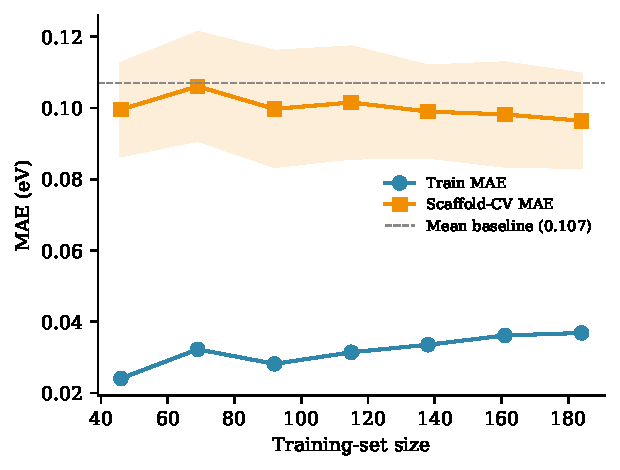
\includegraphics[width=0.72\linewidth]{figures/learning_curve.pdf}
  \caption{Scaffold cross-validation learning curve for the headline NTO random
    forest. Shaded band: $\pm 1$ fold standard deviation of the CV-MAE. The CV-MAE
    is flat beyond $n \approx 90$ and remains above the mean-value baseline gap,
    showing the error does not fall with more data of the same provenance.}
  \label{fig:learning}
\end{figure}

\subsection*{S3.3a Holdout-unit controls and the paper-multiplicity test}
\label{sec:holdout_tables}
\Cref{tab:a017_full} gives the full holdout-unit comparison (\num{50} random assignments of
groups to five folds per unit, random forests with \num{400} trees). Ranges are the 2.5th to
97.5th percentiles over assignments and describe fold-assignment variability, not confidence
intervals. On the fixed scaffold split, $\Delta\rho = \num{0.051}$ with a scaffold-cluster
\qty{95}{\percent} interval of \numrange{-0.099}{0.202}; \qty{25.7}{\percent} of the \num{5000} draws
are $\le 0$, so the contrast under scaffold holdout is not resolved on that split.
\Cref{tab:a019} gives the paper-multiplicity results (\num{103} molecules from multi-molecule
papers, \num{128} from single-molecule papers; same \num{50} assignments, molecule versus paper
holdout). The reading is an association: structural near-duplication and laboratory protocol are
both shared within a paper and are not separable here.

\begin{table*}[t]
  \centering
  \caption{Holdout-unit controls (medians over \num{50} assignments). $\Delta$MAE is Morgan minus
    NTO. Ranges: 2.5th--97.5th percentile over assignments.}
  \label{tab:a017_full}
  \footnotesize\setlength{\tabcolsep}{3pt}
  \begin{tabular}{lcccccc}
    \toprule
    Holdout unit & $\Delta\rho$ (range) & $\Delta\rho>0$ & $\rho$ Morgan & $\rho$ NTO & $\Delta$MAE, eV (range) & NTO higher /20 \\
    \midrule
    Source paper & 0.160 (0.073, 0.246) & 50/50 & 0.172 & 0.337 & $-0.0004$ ($-0.0061$, 0.0068) & 19 \\
    Scaffold     & 0.073 (0.007, 0.144) & 49/50 & 0.269 & 0.351 & $-0.0045$ ($-0.0091$, 0.0010) & 11 \\
    Molecule     & 0.055 ($-0.033$, 0.126) & 45/50 & 0.305 & 0.352 & $-0.0081$ ($-0.0157$, $-0.0002$) & 13 \\
    \bottomrule
  \end{tabular}
\end{table*}

\begin{table*}[t]
  \centering
  \caption{Paper-multiplicity test (medians over \num{50} assignments). Sibling pull is the Spearman
    correlation between the out-of-fold prediction and the leave-self-out mean label of the
    same-paper molecules (\num{103} molecules). Last columns: random minus paper holdout, median
    (2.5th--97.5th percentile).}
  \label{tab:a019}
  \footnotesize\setlength{\tabcolsep}{3pt}
  \begin{tabular}{llcccc}
    \toprule
    Model & Quantity & Random & Paper & Random $-$ paper & Range \\
    \midrule
    Morgan & $\rho$, multi-paper (\num{103}) & 0.538 & 0.264 & 0.269 & 0.174, 0.413 \\
    Morgan & $\rho$, single-paper (\num{128}) & 0.097 & 0.099 & $-0.003$ & $-0.121$, 0.139 \\
    Morgan & sibling pull & 0.676 & 0.255 & 0.415 & 0.276, 0.606 \\
    Morgan & MAE, multi-paper (eV) & & & $-0.025$ & $-0.034$, $-0.014$ \\
    NTO    & $\rho$, multi-paper (\num{103}) & 0.483 & 0.446 & 0.040 & $-0.026$, 0.111 \\
    NTO    & $\rho$, single-paper (\num{128}) & 0.243 & 0.245 & $-0.015$ & $-0.101$, 0.084 \\
    NTO    & sibling pull & 0.471 & 0.418 & 0.048 & $-0.014$, 0.138 \\
    NTO    & MAE, multi-paper (eV) & & & $-0.007$ & $-0.013$, 0.001 \\
    \bottomrule
  \end{tabular}
\end{table*}

\subsection*{S3.3b Assumptions behind the noise ceiling}
\label{sec:r2max_assumptions}
The ceiling $R^2_\text{max} = 1 - \overline{\sigma^2_\text{noise}}/\sigma^2_y$ ($\sigma_y = \qty{0.1666}{\electronvolt}$ from the labels) rests on five
assumptions. (i)~The noise is additive and independent of structure. (ii)~Reports are independent;
\qty{57.8}{\percent} of multi-report molecules have zero spread, which may indicate re-citation, and
that would make their standard error too small and $R^2_\text{max}$ too high. (iii)~The multi-report
term uses $\mathrm{SD}/\sqrt{n}$, the standard error of a mean; the standard error of the median is larger, so
this term is a lower bound on the noise. (iv)~The $\sigma_y$ is computed from the labels, not from the prediction file; the difference
is \qty{0.0004}{\electronvolt} and does not change a reported digit. (v)~The bootstrap interval resamples molecules and does not
propagate uncertainty in the noise estimate itself. Under the three single-report noise choices the ceiling is
\num{0.81} (pooled within-molecule SD \qty{0.0856}{\electronvolt}, primary; \numrange{0.68}{0.88}), \num{0.80}
(\qty{0.0905}{\electronvolt}; \numrange{0.65}{0.87}) and \num{0.86} (\qty{0.072}{\electronvolt}; \numrange{0.75}{0.91}), so the model
($R^2 \approx 0.26$) captures about \qtyrange{30}{32}{\percent} of it.

\subsection*{S3.3 Per-feature SHAP attributions}
\Cref{tab:shap} lists the mean absolute TreeSHAP value of every NTO descriptor for
the random forest trained on the \num{231}-molecule set. Attribution concentrates
on a handful of descriptors: the singlet hole--electron overlap $S_\text{he}(S_1)$
alone accounts for \qty{29}{\percent} of the total attribution, and the top five
descriptors ($S_\text{he}(S_1)$, $S_\text{NTO}^{\text{ratio}}$, $f_{S_1}$,
$\Delta r(S_1)$, $S_\text{he}(T_1)$) for \qty{60}{\percent}. The \num{12}
lowest-ranked descriptors together contribute under \qty{3}{\percent}; the two
raw NTO-overlap and the squared-character features are effectively unused. This is
consistent with the main-text finding that the gap is governed by a small number
of donor--acceptor overlap quantities rather than by the full \num{35}-dimensional
descriptor vector.

\begin{table}[htbp]
  \centering
  \caption{Per-feature importance (mean $|\text{SHAP}|$, in meV) of the \num{35}
    NTO descriptors for the random forest on the \num{231}-molecule experimental
    set, ranked high to low. Regenerated by
    \texttt{code/si\_supplementary\_data.py}.}
  \label{tab:shap}
  \small
  \begin{tabular}{lr@{\hskip 2em}lr}
    \toprule
    Descriptor & meV & Descriptor & meV \\
    \midrule
    $S_\text{he}(S_1)$        & 36.9 & $|\Delta\text{CT}|$            & 1.6 \\
    $S_\text{NTO}^{\text{ratio}}$ & 14.5 & hole-on-A$(T_1)$          & 1.5 \\
    $f_{S_1}$                 & 11.5 & $\Delta r(T_1)$               & 1.5 \\
    $\Delta r(S_1)$           &  7.9 & $\text{CT}(S_1)$              & 1.4 \\
    $S_\text{he}(T_1)$        &  6.9 & $|\Delta\lambda_A|$          & 1.3 \\
    $\log|A_{T_1}|$           &  6.9 & $\Delta\text{CT}$            & 1.2 \\
    $\Delta(\Delta r)$        &  4.8 & particle-on-D$(S_1)$         & 0.7 \\
    $\Delta S_\text{he}$      &  4.3 & $\lambda_D(S_1)$             & 0.7 \\
    $|\Delta(\Delta r)|$      &  4.1 & particle-on-D$(T_1)$         & 0.6 \\
    $|\Delta S_\text{he}|$    &  4.0 & $\lambda_A(T_1)$             & 0.6 \\
    $|\Delta\lambda_D|$       &  3.1 & $\lambda_A(S_1)$             & 0.5 \\
    $\log|A_{S_1}|$           &  3.0 & hole-on-A$(S_1)$             & 0.5 \\
    $\Delta\lambda_D$         &  2.6 & $\Delta S_\text{NTO}$        & 0.1 \\
    $\Delta\lambda_A$         &  2.0 & $S_\text{NTO}^{\text{sum}}$  & 0.1 \\
    $\lambda_D(T_1)$          &  2.0 & NTO overlap$(T_1)$           & 0.1 \\
    $\text{CT}(T_1)$          &  1.7 & NTO overlap$(S_1)$           & 0.0 \\
    \multicolumn{2}{l}{} & $|\Delta S_\text{NTO}|$         & 0.0 \\
    \multicolumn{2}{l}{} & $S_\text{NTO}^{\text{prod}}$    & 0.0 \\
    \multicolumn{2}{l}{} & $\text{Char}_\text{diff}^2$    & 0.0 \\
    \bottomrule
  \end{tabular}
\end{table}

The interpretive value of the physics-informed descriptors is visible when their
attribution is placed beside that of the equally accurate Morgan-fingerprint model
(\cref{fig:shapcompare}). The ten highest-attribution NTO descriptors carry
\qty{79}{\percent} of the total and are all named physical quantities; the ten
highest-attribution Morgan bits carry only \qty{30}{\percent}, spread over
\num{2048} anonymous hashed substructure bits that resist mechanistic reading.
Equal predictive accuracy thus buys interpretability only in the NTO
representation. Regenerated by \texttt{code/shap\_morgan\_vs\_nto.py}.

\begin{figure}[H]
  \centering
  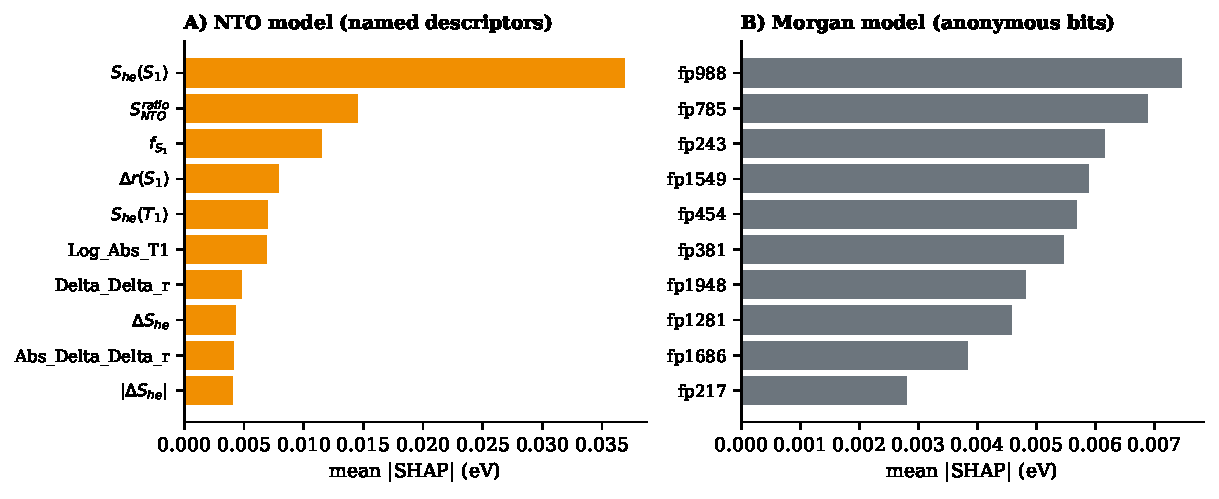
\includegraphics[width=\linewidth]{figures/shap_morgan_vs_nto.pdf}
  \caption{Top-ten SHAP attributions for the two equally accurate models. (A) NTO
    random forest: attribution concentrates on named donor--acceptor overlap and
    charge-transfer descriptors. (B) Morgan random forest: attribution is diffuse
    across anonymous fingerprint bits (\texttt{fp}$n$), which carry no direct
    chemical meaning.}
  \label{fig:shapcompare}
\end{figure}

To test whether this attribution pattern is a stable signal rather than an
artefact of one particular fit, we refit the random forest on \num{200} bootstrap
resamples of the \num{231}-molecule set and recorded the top-five descriptors of
each (\cref{tab:shapboot}). The leading descriptor $S_\text{he}(S_1)$ appears in
the top five of \qty{99.5}{\percent} of resamples; on average \num{3.7} of the five
canonical descriptors recur per resample, and \qty{64.5}{\percent} of resamples
recover at least four of the five. The attribution is therefore reproducible at the
top of the ranking, even though the model's ranking power on the gap itself is
modest; we accordingly read these attributions as mechanistic hypotheses for
experimental test, not validated causal claims. Regenerated by
\texttt{code/shap\_bootstrap\_stability.py}.

\begin{table}[htbp]
  \centering
  \caption{Bootstrap stability of the top-five SHAP descriptors: fraction of
    \num{200} resampled-and-refit models in which each canonical descriptor remains
    in the top five.}
  \label{tab:shapboot}
  \begin{tabular}{lc}
    \toprule
    Descriptor & Top-5 frequency \\
    \midrule
    $S_\text{he}(S_1)$            & \qty{99.5}{\percent} \\
    $S_\text{NTO}^{\text{ratio}}$ & \qty{74.0}{\percent} \\
    $f_{S_1}$                     & \qty{72.0}{\percent} \\
    $\Delta r(S_1)$               & \qty{68.0}{\percent} \\
    $S_\text{he}(T_1)$            & \qty{59.5}{\percent} \\
    \midrule
    Mean top-5 overlap            & 3.7 / 5 \\
    Resamples recovering $\ge 4$  & \qty{64.5}{\percent} \\
    \bottomrule
  \end{tabular}
\end{table}

\subsection*{S3.4 Scaffold-split characterisation}
Because \num{212} Bemis--Murcko scaffolds cover \num{231} molecules,
\qty{92.9}{\percent} of scaffolds are singletons. Scaffold
\texttt{GroupKFold} still differs from a random split in
the way that matters for leakage: by construction no scaffold appears in both
training and test (zero shared groups in every fold), whereas a random split of the
same data leaks \numrange{3}{8} scaffolds per fold across the train/test boundary
(\cref{tab:scaffold}). The numerical effect on difficulty is nonetheless small---the
mean nearest-neighbour Tanimoto similarity between a test molecule and its closest
training molecule falls only from \num{0.615} (random) to \num{0.592} (scaffold)---so
we do not claim the split makes the task dramatically harder; we claim it removes a
specific leakage channel.

That the model learns chemical signal rather than scaffold-group artefacts is
established by a label-permutation test: the target was shuffled \num{1000} times and
the scaffold-CV MAE recomputed under each permutation. The true MAE
(\qty{0.0956}{\electronvolt}) lies far in the left tail of the null distribution
(mean \qty{0.121}{\electronvolt}, SD \qty{0.0043}{\electronvolt}, \qty{95}{\percent}
interval \numrange{0.112}{0.129}), giving $p = 0.001$. Regenerated by
\texttt{code/scaffold\_split\_analysis.py}.

\begin{table}[htbp]
  \centering
  \caption{Scaffold \texttt{GroupKFold} versus a random 5-fold split on the same
    \num{231} molecules. Scaffold splitting removes train/test scaffold overlap; the
    label-permutation test confirms the fitted model is far from the no-signal null.}
  \label{tab:scaffold}
  \footnotesize\setlength{\tabcolsep}{3pt}
  \begin{tabular}{lcc}
    \toprule
    Quantity & Scaffold split & Random split \\
    \midrule
    Shared scaffolds per fold        & 0 (all folds) & 3--8 \\
    Test--train NN Tanimoto (mean)   & 0.592 & 0.615 \\
    \midrule
    \multicolumn{3}{l}{\emph{Label-permutation test (1000 shuffles, scaffold CV)}} \\
    True CV-MAE (eV)                 & \multicolumn{2}{c}{0.0956} \\
    Null CV-MAE: mean (\qty{95}{\percent} CI) (eV) & \multicolumn{2}{c}{0.121 (0.112, 0.129)} \\
    $p$-value (left tail)            & \multicolumn{2}{c}{0.001} \\
    \bottomrule
  \end{tabular}
\end{table}

\subsection*{S3.5 Reproducibility}
The scripts \texttt{code/finalize\_model.py} and
\texttt{code/rebuild\_structural\_model.py} regenerate \cref{tab:model_metrics}
and Fig.~1 of the main text from the benchmark data. The Zenodo
concept DOI \mbox{10.5281/zenodo.17436069} (latest version) holds the archive;
files are listed in S7.

% ─────────────────────────────────────────────────────────────────────────────
\section*{S4. DFT level benchmark}\silabel{S4}{sec:dft_benchmark}
% ─────────────────────────────────────────────────────────────────────────────
Across \num{7} representative emitters in gas and toluene, B3LYP/6-31G(d) and
CAM-B3LYP/def2-TZVP differ in $\Delta E_\text{ST}$ by a mean absolute
\qty{0.30}{\electronvolt} (up to \qty{0.58}{\electronvolt}), with sign reversals
of the relative ordering (e.g.\ DMAC-DPS). This functional dependence limits
claims of agreement across \emph{computed} reference gaps; it is not a physical
error floor for a model trained on measured experimental gaps
(\cref{tab:dft_benchmark}).

\begin{table}[htbp]
  \centering
  \caption{Functional dependence of $\Delta E_\text{ST}$ (eV): B3LYP/6-31G(d)
    vs CAM-B3LYP/def2-TZVP.}
  \label{tab:dft_benchmark}
  \footnotesize\setlength{\tabcolsep}{3pt}
  \begin{tabular}{llccc}
    \toprule
    Molecule & Phase & B3LYP & CAM-B3LYP & $\Delta$ \\
    \midrule
    4CzIPN & gas & 0.192 & 0.361 & +0.169 \\
    4CzIPN & toluene & 0.206 & 0.335 & +0.129 \\
    ACRFLCN & gas & 0.007 & 0.590 & +0.583 \\
    ACRFLCN & toluene & 0.000 & 0.548 & +0.548 \\
    ACRSA & gas & 0.034 & 0.447 & +0.413 \\
    ACRSA & toluene & 0.000 & 0.372 & +0.372 \\
    BACN & gas & 0.524 & 0.991 & +0.467 \\
    BACN & toluene & 0.521 & 0.921 & +0.400 \\
    DMAC-DPS & gas & 0.489 & 0.188 & $-0.301$ \\
    DMAC-DPS & toluene & 0.444 & 0.207 & $-0.237$ \\
    DMAC-TRZ & gas & 0.098 & 0.261 & +0.163 \\
    DMAC-TRZ & toluene & 0.085 & 0.271 & +0.186 \\
    PXZ-NAI & gas & 0.245 & 0.355 & +0.110 \\
    PXZ-NAI & toluene & 0.289 & 0.360 & +0.071 \\
    \bottomrule
  \end{tabular}
\end{table}

A higher-tier check confirms this functional dependence is not an artefact of the
disparate B3LYP/CAM-B3LYP pair. Across six range-separated and hybrid functionals
applied to \num{27} charge-transfer emitters~\cite{Froitzheim2024}, the singlet--triplet gap \emph{estimate}
($E(\text{S}_1^\text{ROKS})-E(\text{S}_1^\text{UKS})\approx\Delta E_\text{ST}/2$)
disagrees per molecule by a median of \qty{0.049}{\electronvolt} (\num{75}th percentile
\qty{0.10}{\electronvolt}, one outlier excluded). Even among modern functionals the
estimate varies at the \qtyrange{0.05}{0.10}{\electronvolt} level; no absolute gap or
experimental agreement is claimed from these data. Extracted by
\texttt{code/parse\_roks\_benchmark.py} from \texttt{results/theoexp\_roks\_energies.csv}.

Three measured sources of variability pertain to different quantities
(\cref{tab:ceiling}); we do \emph{not} combine them into one floor. Only the
experimental label term applies directly to a model trained on the measured
gap. The single-report scatter (A, \qty{0.072}{\electronvolt} RMS) describes
variation between published observations of the same molecule. For the \num{102}
multi-report molecules the median label has an estimated RMS standard error of
\qty{0.049}{\electronvolt}; over all \num{231} molecules, with single-report labels
counted at single-report scatter, label noise is about \qty{0.072}{\electronvolt} RMS,
against a random-forest MAE of \qty{0.096}{\electronvolt} (\qty{95}{\percent} CI
\numrange{0.082}{0.109}). This constrains interpretation of model error but
does not show that the model has reached a noise floor. The
vertical$\rightarrow$adiabatic offset (B, \qty{0.195}{\electronvolt} MAE)
pertains to a computed approximation on \num{14} molecules and is absent
from the 2D model. The functional dependence of a computed gap (C, mean
\qty{0.296}{\electronvolt}) affects comparisons among theoretical
references; it does not set a lower bound on error against experiment. The
capacity tests here did not close the remaining gap
(\cref{tab:capacity}), but other models and representations remain untested.
Component magnitudes are calculated in
\texttt{code/ceiling\_decomposition.py}.

\begin{table*}[t]
  \centering
  \caption{Three measured sources of variability affecting different
    quantities. Only experimental report variability (A) contributes to
    imprecision of the measured target; the RMS standard error of the median
    label is \qty{0.049}{\electronvolt} for the \num{102} multi-report molecules,
    and label noise over all \num{231} is about \qty{0.072}{\electronvolt} RMS. B concerns the
    vertical-to-adiabatic computational approximation, and C concerns
    the choice of functional for a computed gap. They cannot be added into
    an experimental error floor.}
  \label{tab:ceiling}
  \small
  \begin{tabular}{p{0.02\columnwidth}p{0.62\columnwidth}c}
    \toprule
    & Source (what it bounds) & Magnitude (eV) \\
    \midrule
    A & Single-report scatter about the median --- applies to the experimental target (RMS) & 0.072 \\
    B & Vertical$\rightarrow$adiabatic descriptor offset --- largely additive, ranking mostly preserved ($n = 14$); not a target floor (MAE) & 0.195 \\
    C & Functional dependence of the computed reference --- bounds computed-gap agreement only (mean) & 0.296 \\
    \midrule
    & Observed random-forest MAE & 0.096 \\
    & Mean-value baseline & 0.107 \\
    \bottomrule
  \end{tabular}
\end{table*}

\subsection*{S4.1 Vertical versus adiabatic gap}
The NTO descriptors are evaluated at the ground-state (vertical) geometry. To bound
the error this introduces relative to a relaxed (adiabatic) treatment, we recomputed
$\Delta E_\text{ST}$ for \num{14} representative emitters in gas and toluene at
CAM-B3LYP/def2-TZVP (D3BJ, RIJCOSX) with excited-state geometry optimisation in
ORCA, and compared with the vertical sTDA-xTB values (\cref{tab:adiabatic}). Over the
\num{27} converged points the vertical gap deviates from the adiabatic reference by a
mean absolute \qty{0.195}{\electronvolt} (RMSE \qty{0.245}{\electronvolt}, worst case
\qty{0.548}{\electronvolt} for 2CzTPE). The deviation is dominated by an additive offset
rather than by reordering: a linear fit of adiabatic on vertical gives slope \num{1.00}
and intercept \qty{0.07}{\electronvolt} ($R^2 = 0.70$), with rank correlation
Spearman $\rho = 0.71$. The residual is not negligible (RMS
\qty{0.245}{\electronvolt}, signed deviations of both signs) and $n = \num{14}$ cannot
settle how much of it is systematic. Geometry relaxation therefore shifts the absolute
scale while leaving the ordering---on which the triage use depends---largely intact.
Regenerated by \path{code/adiabatic_validation_analysis.py} from
\path{results/vertical_vs_adiabatic_comparison.csv}.

\begin{table}[htbp]
  \centering
  \caption{Vertical (sTDA-xTB, ground-state geometry) versus adiabatic
    (CAM-B3LYP/def2-TZVP, excited-state optimisation) $\Delta E_\text{ST}$ (eV) for
    \num{14} emitters. $\Delta = $ adiabatic $-$ vertical. Summary: MAE
    \qty{0.195}{\electronvolt}, slope \num{1.00}, intercept \qty{0.07}{\electronvolt},
    $R^2 = 0.70$, $\rho = 0.71$.}
  \label{tab:adiabatic}
  \footnotesize
  \begin{tabular}{llccc}
    \toprule
    Molecule & Phase & Vertical & Adiabatic & $\Delta$ \\
    \midrule
    4CzIPN & gas & 0.361 & 0.402 & $+0.041$ \\
    4CzIPN & toluene & 0.335 & 0.436 & $+0.101$ \\
    DMAC-TRZ & gas & 0.261 & 0.442 & $+0.181$ \\
    DMAC-TRZ & toluene & 0.271 & 0.638 & $+0.367$ \\
    DMAC-DPS & gas & 0.188 & 0.385 & $+0.197$ \\
    DMAC-DPS & toluene & 0.207 & 0.558 & $+0.351$ \\
    PXZ-NAI & gas & 0.355 & 0.243 & $-0.112$ \\
    PXZ-NAI & toluene & 0.360 & 0.491 & $+0.131$ \\
    TPA-APy & gas & 0.876 & 0.753 & $-0.123$ \\
    TPA-APy & toluene & 0.765 & 0.895 & $+0.130$ \\
    BACN & gas & 0.991 & 1.129 & $+0.138$ \\
    BACN & toluene & 0.921 & 1.063 & $+0.142$ \\
    BMZ-TZ & gas & 0.938 & 0.410 & $-0.528$ \\
    BMZ-TZ & toluene & 0.933 & 0.700 & $-0.233$ \\
    2CzPN & gas & 0.613 & 0.560 & $-0.053$ \\
    2CzPN & toluene & 0.621 & 0.652 & $+0.031$ \\
    APPT-PXZ & gas & 0.350 & 0.331 & $-0.019$ \\
    2PXZP & gas & 0.467 & 0.384 & $-0.083$ \\
    2PXZP & toluene & 0.485 & 0.639 & $+0.154$ \\
    ACRSA & gas & 0.447 & 0.204 & $-0.243$ \\
    ACRSA & toluene & 0.372 & 0.677 & $+0.305$ \\
    ACRFLCN & gas & 0.590 & 0.302 & $-0.288$ \\
    ACRFLCN & toluene & 0.548 & 0.576 & $+0.028$ \\
    2CzTPE & gas & 1.143 & 1.691 & $+0.548$ \\
    2CzTPE & toluene & 1.042 & 1.535 & $+0.493$ \\
    BBPA & gas & 1.521 & 1.641 & $+0.120$ \\
    BBPA & toluene & 1.433 & 1.562 & $+0.129$ \\
    \bottomrule
  \end{tabular}
\end{table}

\subsection*{S4.2 Triplet manifold (T1--T2)}\label{sec:triplet_manifold}
A small $S_1$--$T_1$ gap does not guarantee fast reverse intersystem crossing; the
$T_1$--$T_2$ splitting and the wider triplet manifold matter too~\cite{Keruckiene2024}.
The same vertical CAM-B3LYP/def2-TZVP TD-DFT calculations that supplied the adiabatic
benchmark also resolve ten triplet roots, so we report $T_1$ and $T_2$ directly
(\cref{tab:manifold}). Across the \num{27} converged emitter--phase points the $T_1$--$T_2$
gap ranges from \qty{0.018}{\electronvolt} (4CzIPN) to \qty{1.50}{\electronvolt} (BBPA),
mean \qty{0.41}{\electronvolt}; \num{13} of \num{27} fall below \qty{0.3}{\electronvolt}.
The manifold therefore varies widely \emph{among molecules with similar $\Delta E_\text{ST}$}
(e.g.\ DMAC-DPS and DMAC-TRZ have near-equal $S_1$--$T_1$ gaps but $T_1$--$T_2$ of
\qtyrange{0.06}{0.26}{\electronvolt}), which is exactly the information a scalar
$\Delta E_\text{ST}$ triage cannot encode and a direction where the excited-state pipeline
adds genuine value. Regenerated by \texttt{code/extract\_triplet\_manifold.py} from the
\texttt{orca\_package} outputs.

\begin{table}[htbp]
  \centering
  \caption{Vertical CAM-B3LYP/def2-TZVP TDA energies (eV): $S_1$, $T_1$, $T_2$, the
    singlet--triplet gap $\Delta E_\text{ST}=S_1-T_1$, and the triplet-manifold gap
    $T_1$--$T_2$, for \num{14} emitters in gas and toluene.}
  \label{tab:manifold}
  \scriptsize
  \begin{tabular}{llccccc}
    \toprule
    Molecule & Phase & $S_1$ & $T_1$ & $T_2$ & $\Delta E_\text{ST}$ & $T_1$--$T_2$ \\
    \midrule
    2CzPN & gas & 3.652 & 3.039 & 3.464 & 0.613 & 0.425 \\
    2CzPN & toluene & 3.632 & 3.011 & 3.459 & 0.621 & 0.448 \\
    2CzTPE & gas & 3.496 & 2.353 & 2.767 & 1.143 & 0.414 \\
    2CzTPE & toluene & 3.411 & 2.369 & 2.788 & 1.042 & 0.419 \\
    2PXZP & gas & 3.292 & 2.825 & 3.080 & 0.467 & 0.255 \\
    2PXZP & toluene & 3.343 & 2.858 & 3.139 & 0.485 & 0.281 \\
    4CzIPN & gas & 3.377 & 3.016 & 3.050 & 0.361 & 0.034 \\
    4CzIPN & toluene & 3.343 & 3.008 & 3.026 & 0.335 & 0.018 \\
    ACRFLCN & gas & 3.597 & 3.007 & 3.548 & 0.590 & 0.541 \\
    ACRFLCN & toluene & 3.546 & 2.998 & 3.536 & 0.548 & 0.538 \\
    ACRSA & gas & 3.769 & 3.322 & 3.513 & 0.447 & 0.191 \\
    ACRSA & toluene & 3.746 & 3.374 & 3.500 & 0.372 & 0.126 \\
    APPT-PXZ & gas & 2.701 & 2.351 & 2.734 & 0.350 & 0.383 \\
    BACN & gas & 3.713 & 2.722 & 3.533 & 0.991 & 0.811 \\
    BACN & toluene & 3.629 & 2.708 & 3.503 & 0.921 & 0.795 \\
    BBPA & gas & 3.553 & 2.032 & 3.525 & 1.521 & 1.493 \\
    BBPA & toluene & 3.458 & 2.025 & 3.526 & 1.433 & 1.501 \\
    BMZ-TZ & gas & 3.730 & 2.792 & 3.180 & 0.938 & 0.388 \\
    BMZ-TZ & toluene & 3.896 & 2.963 & 3.142 & 0.933 & 0.179 \\
    DMAC-DPS & gas & 3.637 & 3.449 & 3.508 & 0.188 & 0.059 \\
    DMAC-DPS & toluene & 3.678 & 3.471 & 3.538 & 0.207 & 0.067 \\
    DMAC-TRZ & gas & 3.509 & 3.248 & 3.504 & 0.261 & 0.256 \\
    DMAC-TRZ & toluene & 3.533 & 3.262 & 3.509 & 0.271 & 0.247 \\
    PXZ-NAI & gas & 2.688 & 2.333 & 2.836 & 0.355 & 0.503 \\
    PXZ-NAI & toluene & 2.650 & 2.290 & 2.829 & 0.360 & 0.539 \\
    TPA-APy & gas & 3.555 & 2.679 & 2.823 & 0.876 & 0.144 \\
    TPA-APy & toluene & 3.425 & 2.660 & 2.795 & 0.765 & 0.135 \\
    \bottomrule
  \end{tabular}
\end{table}

To read the manifold across the whole corpus rather than the \num{14}-molecule ORCA
subset, we extracted $T_1$ and $T_2$ for all \num{231} emitters from the cheaper
sTDA-xTB pipeline (\texttt{code/extract\_t1\_t2\_rerun.py}; \num{231}/\num{231}
converged, \texttt{results/t1\_t2\_full.csv}). The full-corpus $T_1$--$T_2$ gap has median
\qty{0.14}{\electronvolt} (mean \qty{0.24}{\electronvolt}), and \qty{74}{\percent} of
emitters fall below the \qty{0.3}{\electronvolt} region where a near-degenerate second
triplet can open competing non-radiative channels (\cref{fig:t1t2dist}). Most
low-gap candidates therefore remain exposed to inefficient reverse intersystem
crossing---a hazard a scalar $S_1$--$T_1$ triage cannot see.

This full-corpus manifold must be read \emph{qualitatively only}. Benchmarking the
sTDA-xTB $T_1$--$T_2$ gap against the CAM-B3LYP reference on the six overlapping
molecules gives a mean absolute deviation of \qty{0.237}{\electronvolt}
(Spearman $\rho = 0.43$, $p = 0.40$; \cref{tab:manifold_val}), so the two methods agree
on neither magnitude nor rank at a useful level. Quantitative ranking on RISC propensity
still requires the higher-level calculation; the sTDA manifold serves only to flag that
the triplet-manifold hazard is widespread, not to order candidates by it.

\begin{table}[htbp]
  \centering
  \caption{sTDA-xTB versus CAM-B3LYP $T_1$--$T_2$ gap (eV) for the six molecules present
    in both sets. Independent methods; the comparison is genuine (fresh GFN2 geometries).
    Summary: MAE \qty{0.237}{\electronvolt}, Spearman $\rho = 0.43$ ($p = 0.40$, $n = 6$).}
  \label{tab:manifold_val}
  \small
  \begin{tabular}{lcc}
    \toprule
    Molecule & sTDA-xTB & CAM-B3LYP \\
    \midrule
    2CzPN    & 0.169 & 0.425 \\
    2PXZP    & 0.004 & 0.255 \\
    4CzIPN   & 0.073 & 0.034 \\
    ACRSA    & 0.006 & 0.191 \\
    DMAC-DPS & 0.011 & 0.059 \\
    PXZ-NAI  & 1.146 & 0.503 \\
    \bottomrule
  \end{tabular}
\end{table}

\begin{figure}[htbp]
  \centering
  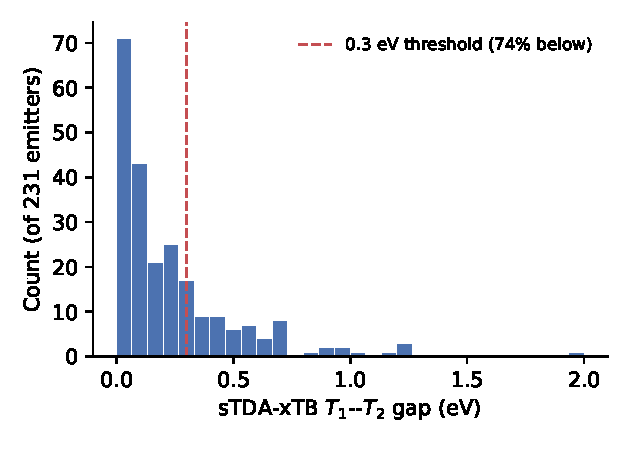
\includegraphics[width=0.72\columnwidth]{figures/t1_t2_distribution.pdf}
  \caption{Distribution of the sTDA-xTB $T_1$--$T_2$ gap across all \num{231} emitters.
    \qty{74}{\percent} fall below \qty{0.3}{\electronvolt} (dashed line). Read
    qualitatively only (\cref{tab:manifold_val}).}
  \label{fig:t1t2dist}
\end{figure}

\subsection*{S4.3 Range-separated TD-DFT reference gap}\label{sec:tddft_reference}

Referee comment on the original submission held that the semi-empirical
sTDA gap understates what a proper range-separated TD-DFT calculation would
achieve. We tested this directly. Vertical $\Delta E_\text{ST}$ was computed for all
\num{231} benchmark molecules at wB97X-D4/def2-SVP with RIJCOSX and the
Tamm--Dancoff approximation (ORCA~6~\cite{Neese2020}; \texttt{nroots}~8, triplets
included), at the GFN2-xTB ground-state geometry, with
$\Delta E_\text{ST} = E(S_1) - E(T_1)$. All \num{231}/\num{231} jobs terminated
normally with all states parsed and no inverted gaps; the run cost
\num{609} core-hours (measured: \qty{76.2}{\hour} elapsed on \num{8} processes; median
\qty{16.1}{\minute} per molecule, slowest \qty{2.1}{\hour}; wall
$\propto$~atoms$^{1.89}$). Per-molecule gaps and timings are in
\texttt{results/tddft\_reference\_231.csv}; the head-to-head analysis is
\texttt{results/ref1\_tddft\_gap.json}, produced by \texttt{code/ref1\_tddft\_gap.py}
on the same experimental labels, SMILES, NTO features and scaffold
\texttt{GroupKFold} folds as \cref{tab:model_metrics}.

The raw TD-DFT gap overestimates the measured gap by a systematic
\qty{+0.654}{\electronvolt} (TD-DFT mean \qty{0.803}{\electronvolt},
SD \qty{0.248}{}; experiment mean \qty{0.149}{\electronvolt}, SD \qty{0.167}{}),
more than triple the \qty{+0.221}{\electronvolt} sTDA offset. sTDA and TD-DFT
gaps agree only moderately with each other ($r = 0.461$, $\rho = 0.402$, mean
shift \qty{+0.433}{\electronvolt}). An in-fold degree-1 calibration
($a\,g + b$, fitted per training fold on $\approx\!185$ molecules, no test leak)
removes the offset. \cref{tab:tddft_headtohead} lists every predictor on the
common folds; \cref{tab:tddft_paired} the paired MAE differences (2000-resample
bootstrap on identical folds plus Wilcoxon signed-rank on paired absolute
errors).

\begin{table*}[htbp]
  \centering
  \caption{TD-DFT reference gap versus semi-empirical gap and structure-only
    random forests, all on the same \num{231}-molecule scaffold
    \texttt{GroupKFold}($k=5$) folds. B rows are single-quantity predictors;
    M rows are random forests (\num{400} trees). ``Calibrated'' = in-fold linear
    fit requiring experimental training labels.}
  \label{tab:tddft_headtohead}
  \small
  \begin{tabular}{llccccc}
    \toprule
    & Predictor & MAE (eV) & RMSE (eV) & $R^2$ & $r$ & $\rho$ \\
    \midrule
    B0 & Mean baseline                 & 0.107 & 0.167 & $-0.01$  & $-0.11$ & $-0.06$ \\
    B1 & Raw sTDA gap                  & 0.251 & 0.299 & $-2.22$  & 0.32 & 0.24 \\
    B3 & Raw TD-DFT gap                & 0.654 & 0.694 & $-16.3$  & 0.43 & 0.38 \\
    B2 & Calibrated sTDA gap           & 0.104 & 0.160 & 0.08     & 0.29 & 0.23 \\
    B4 & Calibrated TD-DFT gap         & 0.099 & 0.152 & 0.17     & 0.41 & 0.37 \\
    \midrule
    M1 & RF Morgan (structure only)    & 0.091 & 0.142 & 0.27 & 0.55 & 0.31 \\
    M2 & RF NTO (energy-free)          & 0.096 & 0.144 & 0.25 & 0.50 & 0.36 \\
    M5 & RF NTO $+$ TD-DFT gap         & 0.092 & 0.140 & 0.29 & 0.54 & 0.40 \\
    M6 & RF Morgan $+$ TD-DFT gap      & 0.087 & 0.138 & 0.31 & 0.58 & 0.37 \\
    M7 & RF NTO $+$ sTDA $+$ TD-DFT    & 0.093 & 0.141 & 0.29 & 0.54 & 0.39 \\
    \bottomrule
  \end{tabular}
\end{table*}

\begin{table*}[htbp]
  \centering
  \caption{Paired MAE difference on identical folds (positive = the TD-DFT gap
    helps). CI from \num{2000} paired bootstrap resamples; $p$ from the Wilcoxon
    signed-rank test on paired absolute errors.}
  \label{tab:tddft_paired}
  \small
  \begin{tabular}{lccc}
    \toprule
    Comparison & $\Delta$MAE /eV & \qty{95}{\percent} CI /eV & Wilcoxon $p$ \\
    \midrule
    M6 vs M1 (Morgan $+$ gap)      & $+0.0039$ & $[+0.0004,\,+0.0071]$ & 0.016 \\
    M5 vs M2 (NTO $+$ gap)         & $+0.0032$ & $[+0.0008,\,+0.0058]$ & 0.013 \\
    B4 vs B0 (calib.\ gap vs mean) & $+0.0085$ & $[+0.0002,\,+0.0164]$ & 0.006 \\
    B4 vs M1 (calib.\ gap vs RF)   & $-0.0075$ & $[-0.0205,\,+0.0061]$ & 0.28 \\
    B3 vs B1 (raw TD-DFT vs sTDA)  & $-0.403$  & $[-0.431,\,-0.375]$   & \num{1e-37} \\
    \bottomrule
  \end{tabular}
\end{table*}

Read raw, a higher level of theory is worse, not better: the range-separated
TDA gap is the least accurate predictor in the study, driven by a large
fixed exchange-splitting overestimate. It does track experiment better in rank
($r$ \num{0.32}~to~\num{0.43} from sTDA to TD-DFT) and, once calibrated on
experimental labels, in MAE (\qty{0.099}{\electronvolt}, below the mean baseline
but not the structure-only forest). Added as one random-forest feature it gives
the only physics contribution in this work that clears a paired test
(M6 vs M1, M5 vs M2), a \qty{4}{\percent} MAE reduction for \num{609}
core-hours. Caveats: gas-phase vertical values only (no solvent, no
excited-state relaxation); the \qty{+0.654}{\electronvolt} bias is specific to
wB97X-D4/def2-SVP/TDA; def2-SVP is a small basis, though the systematic offset
is expected to persist at a larger basis for a range-separated hybrid; TDA raises triplet
energies relative to full TD-DFT, widening the gap, and was the deliberate stable
choice; the M5/M6 gains ($\approx$\qty{0.003}{}--\qty{0.004}{\electronvolt}) are
real by the paired test but small against the \qty{0.072}{\electronvolt}
single-report label scatter.

% ─────────────────────────────────────────────────────────────────────────────
\section*{S5. Substructure-filtered extended library}\silabel{S5}{sec:library}
% ─────────────────────────────────────────────────────────────────────────────
An extended set of \num{22194} structures was obtained by screening the PubChem
CID--SMILES collection for compounds carrying both a donor motif (carbazole,
phenothiazine, phenoxazine, acridine, diphenylamine, triphenylamine or dimethylaniline)
and an acceptor motif (triazine, benzonitrile, pyridine, pyrimidine, quinoxaline,
benzothiadiazole, naphthoquinone or a cyano group), under the constraints
MW $<\qty{900}{\dalton}$, $\geq 2$ aromatic rings and $\geq 1$ N/O/S heteroatom.
The screen is in \texttt{code/build\_shortlist.py} and the screening script in the deposit.
It is a substructure filter over an existing database, not a combinatorial enumeration
of fragment pairs, and the distinction matters for how the set should be read: every
member satisfies the donor--acceptor pattern test, but the matches are dominated by the
weaker motifs (dimethylaniline in \qty{85}{\percent} and pyridine in \qty{59}{\percent}
of the \num{100} lowest-predicted structures, against carbazole in \num{2} and triazine
in \num{3}). The set also inherits the composition of the source database rather than of
a designed emitter series: \qty{97}{\percent} of those structures carry a halogen and
\qty{53}{\percent} a stereocentre, and enantiomer pairs appear as separate entries with
identical predicted gaps, which a 2D fingerprint cannot distinguish. Candidates were
ranked by a rule-based TADF score
\begin{equation}
  \begin{aligned}
    \text{TADF score} ={}& 0.35\,f_\text{MW} + 0.25\,f_\text{LogP} \\
                    & {}+ 0.20\,f_\text{rings} + 0.20\,f_\text{hetero},
  \end{aligned}
  \label{eq:tadf_score}
\end{equation}
with each $f_i\in[0,1]$ a normalised feature score based on established design
heuristics~\cite{Liu2012,Uoyama2012,Wong2017}. The score is a coarse
synthesis-planning filter, \emph{not} a calibrated $\Delta E_\text{ST}$ predictor.
The random-forest model trained on the labelled benchmark is applied to this set only to
obtain split-conformal prediction intervals (S6.7); no candidate is put forward on the
strength of its predicted gap. These are
synthesis-planning leads only: they are not quantum-validated, and the heuristic
score is not a calibrated $\Delta E_\text{ST}$ predictor. Property distributions
of the filtered set versus the top-scoring subset are shown in
\cref{fig:library_analysis}.

\begin{figure}[htbp]
  \centering
  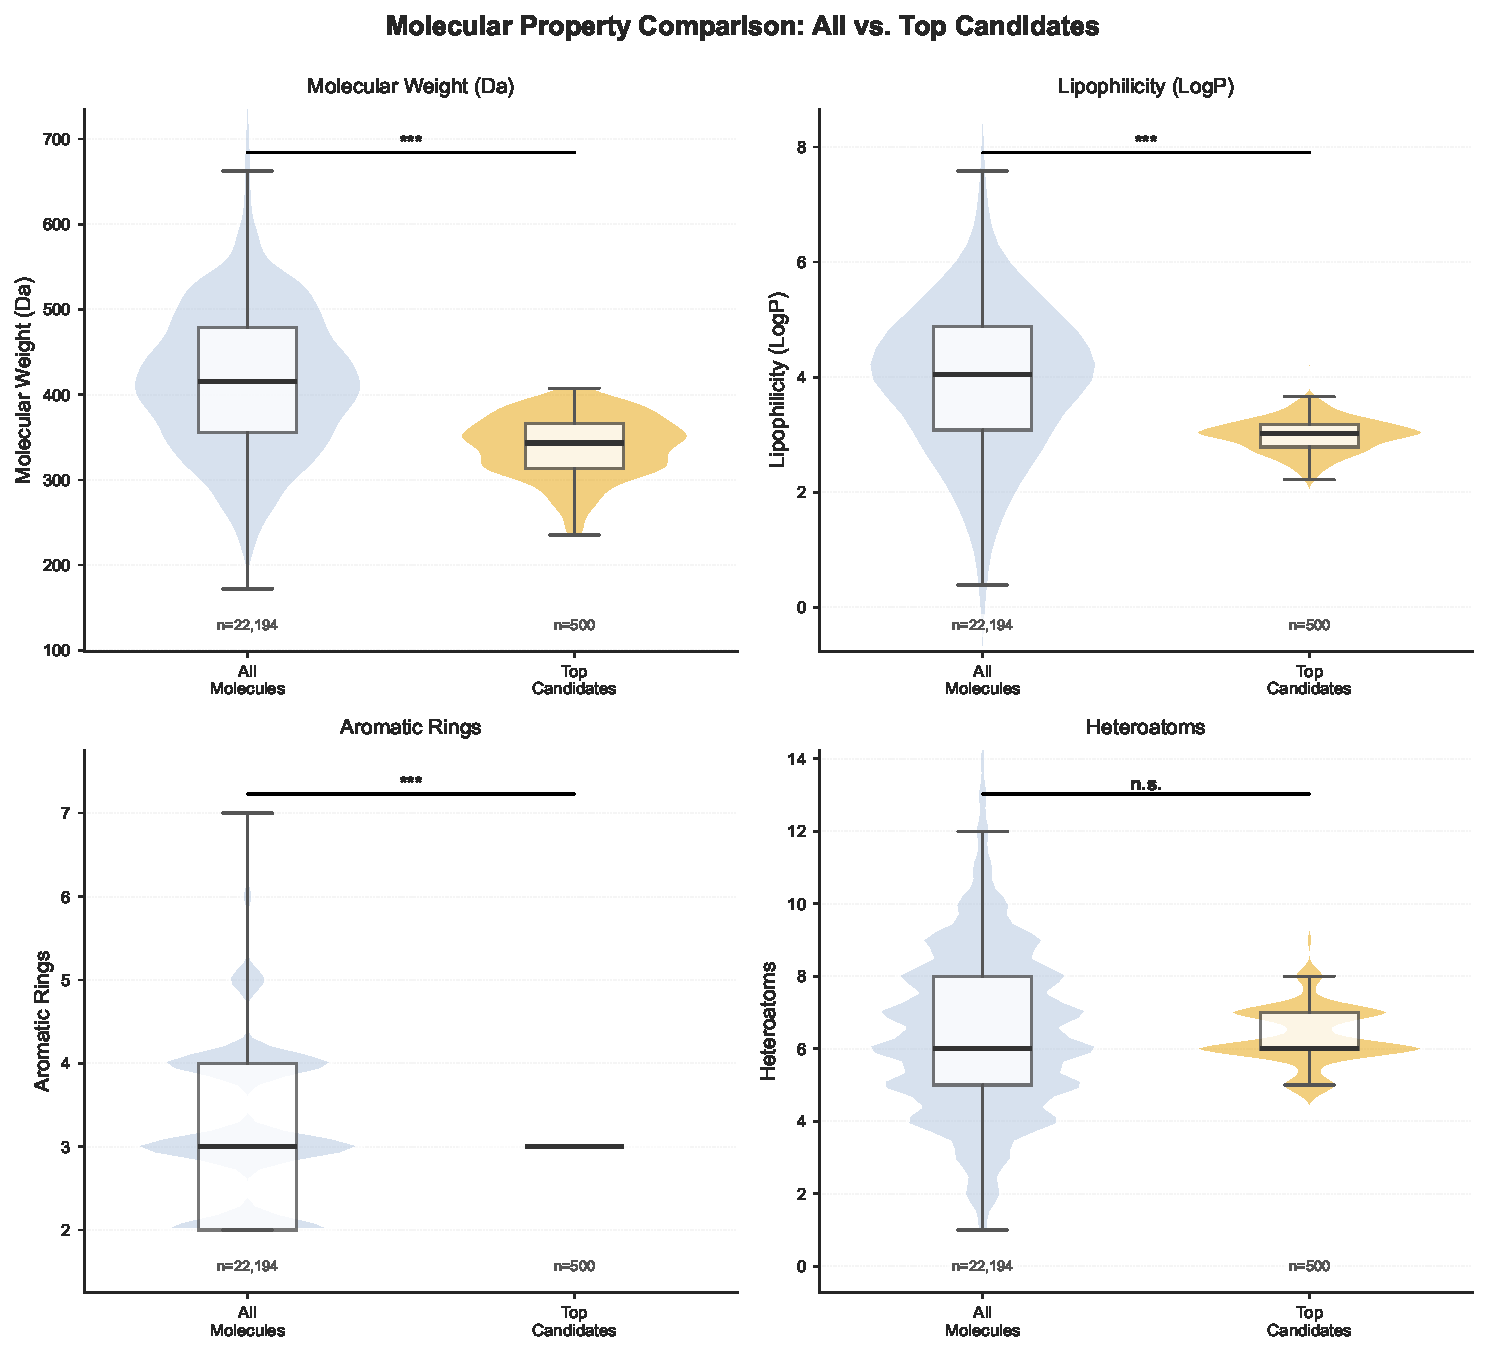
\includegraphics[width=\linewidth]{figures/property_comparison.pdf}
  \caption{Property distributions of the filtered library (\num{22194}
    PubChem structures passing the donor--acceptor substructure screen, grey) versus the
    top \num{500} by heuristic TADF score
    (blue). Enrichment toward lower molecular weight reflects the scoring rule;
    these are unvalidated leads, not predicted emitters.}
  \label{fig:library_analysis}
\end{figure}

We additionally ranked the full library with the calibrated structure-only
Morgan-FP model and attached a split-conformal \qty{90}{\percent} prediction
interval to every prediction (mean half-width \qty{0.18}{\electronvolt},
empirical coverage \num{0.89}). No ranked shortlist is deposited: for the leading
candidates the predicted gap is \qtyrange{0.02}{0.05}{\electronvolt} while the full
interval width is about \num{7.6} times as large (half-width \num{3.8} times), and the lower bound of
every one of the \num{100} lowest-predicted intervals falls below zero. At this
accuracy the conformal procedure does not support selection at the
single-molecule level, and no device-level quantity is predicted.

% ─────────────────────────────────────────────────────────────────────────────
\section*{S6. Robustness analyses}
% ─────────────────────────────────────────────────────────────────────────────

\subsection*{S6.1 Cluster cross-validation}
Because \qty{92.9}{\percent} of scaffolds are singletons, we built non-singleton groups
by Butina clustering (Morgan Tanimoto distance) and ran cluster-grouped CV across a
cutoff scan (\cref{tab:clustercv}). Even at
the coarsest grouping (\num{70} clusters, largest \num{38} molecules), the MAE
(\qty{0.099}{\electronvolt}) sits between scaffold-CV (\qty{0.096}{\electronvolt}) and
random-CV (\qty{0.106}{\electronvolt}), a spread of \qty{0.010}{\electronvolt}. Performance is
therefore \emph{stable across validation schemes}: the headline number is not an artefact of
singleton scaffolds. Regenerated by \texttt{code/cluster\_cv\_analysis.py}.

\begin{table}[htbp]
  \centering
  \caption{Cluster-grouped CV of the headline NTO RF across Butina distance cutoffs,
    with scaffold and random CV for reference.}
  \label{tab:clustercv}
  \footnotesize
  \begin{tabular}{lcccc}
    \toprule
    Grouping & \#groups & largest & MAE (eV) & $\rho$ \\
    \midrule
    Butina 0.3 & 186 & 7  & 0.100 & 0.35 \\
    Butina 0.4 & 153 & 10 & 0.100 & 0.38 \\
    Butina 0.5 & 111 & 15 & 0.104 & 0.31 \\
    Butina 0.6 & 70  & 38 & 0.099 & 0.40 \\
    \midrule
    Scaffold (headline) & 212 & --- & 0.096 & 0.36 \\
    Random 5-fold       & --- & --- & 0.106 & 0.34 \\
    \bottomrule
  \end{tabular}
\end{table}

\subsection*{S6.2 Dimensionality and model capacity}
Two checks address the charge that a \num{2048}-bit fingerprint over-parameterises a
\num{231}-molecule set. First, shrinking the fingerprint to \num{1024} or \num{512} bits
leaves the MAE and the (negative) lower $R^2$ confidence bound essentially unchanged
(\cref{tab:capacity}, top), so the negative $R^2$ tail is intrinsic to the low
variance-explained on this target, not a width artefact; the lowest-dimensional regularised
model (NTO + ElasticNet) brings the lower bound closest to zero ($-0.03$) but does not lift
it. Second, no higher- or different-capacity learner beats the random forest under the same
scaffold CV (\cref{tab:capacity}, bottom): gradient boosting, an MLP and an SVR are all
worse. Model capacity is not the limiting factor. Retraining on the \num{208} molecules whose
inter-report standard deviation is $\le\qty{0.05}{\electronvolt}$ does not lower the MAE
(\qty{0.106}{\electronvolt}). That subset is a weak test, because \num{129} of those
\num{208} molecules have no replicate at all and enter with SD~$=0$ by construction, so
only \num{23} molecules are actually excluded. Conditioning instead on molecules that
carry replicates, and reading the error off the same out-of-fold predictions, the model
achieves \qty{0.074}{\electronvolt} on the \num{79} whose reports agree to
$\le\qty{0.05}{\electronvolt}$, \qty{0.106}{\electronvolt} on the \num{23} whose
reports disagree, and \qty{0.107}{\electronvolt} on the \num{129} whose label precision
cannot be measured. The constant predictor scores \qty{0.074}{}, \qty{0.107}{} and
\qty{0.110}{\electronvolt} on the same strata, respectively, so the comparison carries
no information about label quality. Regenerated by \texttt{code/dimensionality\_check.py} and
\texttt{code/capacity\_and\_noise\_ceiling.py}.

\begin{table}[htbp]
  \centering
  \caption{Top: fingerprint-width sweep (RF) — MAE and \qty{95}{\percent} bootstrap $R^2$
    CI. Bottom: alternative learners under the same scaffold CV. None beats the RF.}
  \label{tab:capacity}
  \footnotesize
  \begin{tabular}{lcc}
    \toprule
    Setting & MAE (eV) & $R^2$ (\qty{95}{\percent} CI) \\
    \midrule
    Morgan 512 (RF)   & 0.098 & 0.15 ($-0.44$, 0.46) \\
    Morgan 1024 (RF)  & 0.096 & 0.24 ($-0.25$, 0.51) \\
    Morgan 2048 (RF)  & 0.091 & 0.27 ($-0.19$, 0.53) \\
    NTO + ElasticNet  & 0.102 & 0.10 ($-0.03$, 0.17) \\
    \midrule
    RandomForest (headline) & 0.096 & --- \\
    HistGradientBoosting    & 0.105 & --- \\
    MLP (100, 50)           & 0.169 & --- \\
    SVR (RBF)               & 0.120 & --- \\
    ElasticNet              & 0.102 & --- \\
    \bottomrule
  \end{tabular}
\end{table}

\subsection*{S6.3 SHAP cross-check by permutation importance}
An independent, model-agnostic permutation-importance analysis (held-out \qty{30}{\percent},
\num{50} repeats) ranks the singlet hole--electron overlap $S_\text{he}(S_1)$ \emph{first},
in agreement with TreeSHAP; two of the SHAP top-five recur in the permutation top-five. The
leading attribution is thus corroborated by two methods, while the lower-ranked tail is not
--- consistent with our restriction of mechanistic reading to the dominant descriptor.
Regenerated by \texttt{code/permutation\_importance\_check.py}.

\subsection*{S6.4 Enrichment curve and calibrated operating points}
The main-text enrichment curve reports precision (fraction of selected molecules with experimental
gap $\le\qty{0.10}{\electronvolt}$) against screening budget. Enrichment peaks at
\num{1.37}$\times$ over the \qty{49}{\percent} base rate around the top \qtyrange{5}{20}{\percent}
and does not improve at more aggressive cuts (the top \qty{1}{\percent} is two molecules). A
split-conformal calibration gives a \qty{90}{\percent} interval half-width of
\qty{0.178}{\electronvolt} (empirical coverage \num{0.892}). These
intervals convey uncertainty but are too wide to identify an individual
low-gap emitter reliably. Regenerated by \texttt{code/enrichment\_curve.py}.

\subsection*{S6.5 Multi-criteria triage}
A small $S_1$--$T_1$ gap is necessary but not sufficient for efficient delayed
fluorescence: the emitter must also be optically bright and free of a near-degenerate
second triplet. We therefore composed the predicted gap with two auxiliary structure-level
filters---oscillator strength $f_{S_1}\ge\num{0.01}$ (\num{209}/\num{231} pass;
\texttt{code/oscillator\_strength\_model.py}) and sTDA $T_1$--$T_2 > \qty{0.10}{\electronvolt}$
(\cref{tab:manifold_val})---leaving \num{131} molecules that clear all three
(\texttt{code/multi\_criteria\_triage.py}). Ranking within this pool raises the top-\qty{5}{\percent}
precision for low-gap emitters from \num{0.58} (gap alone) to \num{0.71}, i.e.\ enrichment
\num{1.18}$\rightarrow$\num{1.45}$\times$; the two curves converge by the top \qty{50}{\percent}.
The gain is real but small and rests on only a handful of molecules at the sharpest cut, so we
read the multi-criteria filter not as a precision gain but as a physically motivated way
to discard the \qty{43}{\percent} of low-gap candidates that are dark or manifold-unsafe---a
decision a scalar-gap triage cannot make. The $T_1$--$T_2$ term inherits the qualitative-only
caveat of \cref{tab:manifold_val}.

\subsection*{S6.6 Dataset expansion stress-test}
To test whether the benchmark is limited by corpus size, we resolved and featurised
\num{624} additional donor--acceptor emitters from the experimental literature
(name-to-structure resolution followed by the identical GFN2-xTB/sTDA natural-transition-orbital
pipeline; \texttt{code/expand\_dataset.py}, \texttt{code/featurize\_nto\_local.py}). After
discarding \num{127} structures already present in the training set, \num{497} genuinely new
molecules extend the corpus to \num{728} (\cref{tab:expansion}). Enlarging the set does
\emph{not} improve structure-only prediction: under the same scaffold CV the MAE rises from
\qty{0.098}{\electronvolt} to \qty{0.124}{\electronvolt} and $R^2$ falls to \num{-0.01} (the
curated-set MAE of \qty{0.098}{\electronvolt} reproduces the headline \qty{0.096}{\electronvolt}
within single-seed variation). Restricting the new molecules to those with replicate
measurements (\num{234} with $\ge\num{2}$ independent reports) recovers part of the loss
(MAE \qty{0.110}{\electronvolt}, $R^2$ \num{0.05}), placing one component of the degradation in
label noise from automated literature extraction. We do not decompose the degradation
further: the added molecules are resolved through a different structure pipeline, so
label quality and chemical diversity are confounded and this design cannot apportion the
loss between them. What the expansion rules out is that the corpus is merely too small. Regenerated by \texttt{code/expansion\_stress\_test.py}.

\begin{table}[htbp]
  \centering
  \caption{Scaffold-CV of the NTO random forest as the corpus is expanded and as
    new-label confidence is tightened. Expansion does not improve accuracy.}
  \label{tab:expansion}
  \footnotesize
  \begin{tabular}{lcccc}
    \toprule
    Corpus & $n$ & MAE (eV) & $R^2$ & $\rho$ \\
    \midrule
    Curated baseline            & 231 & 0.098 & \phantom{$-$}0.18 & 0.34 \\
    + all new                   & 728 & 0.124 & $-0.01$           & 0.16 \\
    + multi-report new ($\ge 2$) & 465 & 0.110 & \phantom{$-$}0.05 & 0.24 \\
    \bottomrule
  \end{tabular}
\end{table}

\subsection*{S6.7 Candidate triage and the filtered library (moved from the main text)}\label{subsec:triage_library}
\paragraph{Candidate prioritisation as a triage filter.}

The model's practical value is as a coarse triage filter: it eliminates the bottom
tier of candidates rather than ordering the viable subset. We quantify this directly. Taking emitters with experimental
$\Delta E_\text{ST}\le\qty{0.10}{\electronvolt}$ as the targets (\qty{49}{\percent}
of the set), the structure-only model's top-ranked candidates are enriched in
targets relative to random selection by \numrange{1.2}{1.4}$\times$
(precision rising from the \qty{49}{\percent} base rate to \qty{60}{\percent} at
the top \num{10}--\num{20} and \qty{68}{\percent} at the top \num{50}); a bootstrap
confidence interval on this cross-validation enrichment, given below, shows the smaller cutoffs are
not statistically distinguishable from chance.
Note that $\Delta E_\text{ST}$ is a necessary but not sufficient condition for TADF
efficiency; emission wavelength matching is a subsequent, independent design step
not addressed by this model.
The filter therefore works, but weakly: it is a coarse
first pass that modestly concentrates good emitters, not a selector. Part of that
weakness is the threshold itself: \qty{0.10}{\electronvolt} is only
\qty{0.03}{\electronvolt} above the \qty{0.072}{\electronvolt} RMS inter-report
scatter (the main-text ceiling subsection), so a molecule's true class membership near that
line is itself uncertain at the level of label noise---tightening the triage
threshold runs directly into the same ceiling that bounds the regression task.
Among well-characterised emitters, DMAC-DPS
(experimental $\Delta E_\text{ST}\approx\qty{0.09}{\electronvolt}$) and PXZ-NAI are
examples of low-gap emitters the filter retains.
Application to a specific lighting niche---horticultural or human-centric---is a
\emph{separate, downstream} step: it requires matching the emission wavelength and
oscillator strength, neither of which this scalar $\Delta E_\text{ST}$ model predicts.
We therefore make no spectral-matching or device-level claim (reverse intersystem
crossing rates and external quantum efficiencies depend on quantities this model does
not resolve, and our earlier device estimates did not survive scrutiny
(main-text limitations paragraph).

\paragraph{A substructure-filtered extended chemical space.}

To indicate the chemical space such triage would operate over, we screened PubChem for
structures carrying both a donor and an acceptor motif, retaining \num{22194}
(main-text Methods, library subsection; molecular weights \qtyrange{172}{899}{\dalton},
\numrange{2}{12} aromatic rings; property distributions in
\cref{fig:library_analysis}). Every member passes the donor--acceptor pattern test,
but the set carries the composition of the source database rather than of a designed
emitter series, and its matches lean on the weaker motifs; it indicates scale, not a
curated design space. We do not deposit a
ranked candidate list. On the filtered set the split-conformal
\qty{90}{\percent} prediction interval spans \qty{0.36}{\electronvolt} (mean
half-width \qty{0.18}{\electronvolt}), about \num{7.6} times the predicted gap, and for
every one of the \num{100} lowest-predicted molecules the interval's lower bound
falls below zero. At this accuracy conformal prediction refuses selection at the
single-molecule level; the filtered set only indicates the scale of the space that the
labelled-data triage would operate over. The heuristic score of
the main-text TADF score equation remains a planning aid, not a calibrated predictor, and the
retained molecules are not quantum-validated.

\paragraph{Quantifying triage utility.}
On held-out labelled molecules the structure-only model enriches the low-gap
class by \numrange{1.2}{1.4}$\times$ over random selection, but a
\qty{95}{\percent} bootstrap confidence interval (\num{5000} resamples over
molecules, the ranking re-derived from the fixed cross-validation out-of-fold predictions within
each resample) shows this holds only at the less aggressive cutoffs. Against the
\qty{49}{\percent} base rate ($\Delta E_\text{ST} \le \qty{0.10}{\electronvolt}$),
top-ranked precision reaches \qty{60}{\percent} at both the top \num{10} and top
\num{20} candidates (enrichment \num{1.22}$\times$, \qty{95}{\percent} CI
\numrange{0.63}{1.89} and \numrange{0.80}{1.70}: both intervals include no
enrichment), and \qty{68}{\percent} at the top \num{50} (\num{1.38}$\times$, CI
\numrange{1.10}{1.60}) or \qty{67.4}{\percent} at the top \qty{20}{\percent} of the
benchmark (\num{1.37}$\times$, CI \numrange{1.08}{1.61}: both intervals exclude no
enrichment). The enrichment is therefore only statistically established at cutoffs
of roughly \num{50} molecules or a fifth of the benchmark; at the ten-to-twenty
candidate scale a laboratory would actually shortlist, it cannot be distinguished
from chance at this sample size. The full enrichment curve
(\cref{fig:enrichment}) peaks near \num{1.37}$\times$ at the top
\qtyrange{5}{20}{\percent} and does not improve at more aggressive cuts; a split-conformal
calibration lets a laboratory fix an operating point at a stated confidence. This
is a statement about the labelled benchmark: the model supports \emph{triage},
not selection, and the interval widths reported above rule out
projecting a hit rate onto the unvalidated filtered library.

\begin{figure}[t]
  \centering
  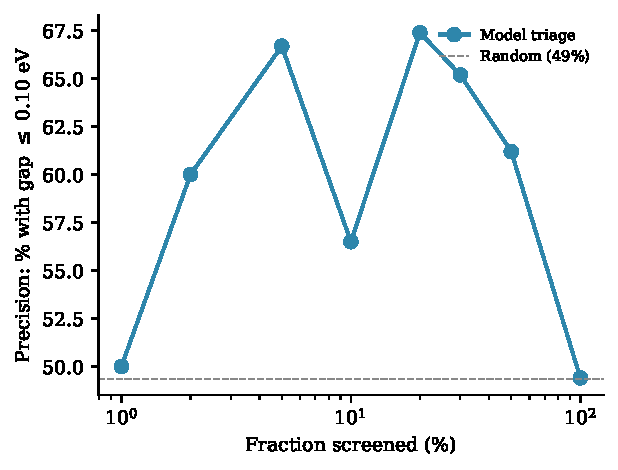
\includegraphics[width=\linewidth]{figures/enrichment_curve.pdf}
  \caption{Triage precision versus fraction of the benchmark screened (log $x$).
    Dashed line: the \qty{49}{\percent} random base rate. Enrichment is real but
    bounded at $\approx 1.3$--$1.4\times$; the top \qty{1}{\percent} is two molecules.}
  \label{fig:enrichment}
\end{figure}

\subsection*{S6.8 Detailed limitations (moved from the main text)}\label{subsec:limitations_si}

This study is bounded in several ways.
(1)~The experimental corpus is heterogeneous (mixed solvents and methods,
\qty{0.072}{\electronvolt} RMS inter-report scatter); a single-source,
solvent-controlled dataset would help separate label variability from
representation error. The estimated noise bound lies well above observed
$R^2$, so a model improvement is not excluded by these data.
(2)~The model predicts a consensus gap, not solvatochromic or
conformer-dependent values.
(3)~We make no quantitative device claims.
Molecule-independent estimates for spin–orbit coupling, $k_\text{RISC}$, and external quantum efficiency, derived from literature medians, were deliberately 
excluded from this analysis.
% An earlier version of this work included
% molecule-independent estimates for spin--orbit coupling, $k_\text{RISC}$, and
% external quantum efficiency derived from literature medians. Following internal peer
% review, these estimates were removed because the inter-molecular variance in these
% quantities exceeds the precision of a scalar estimate by an order of magnitude. We
% view this correction as an illustration of the iterative rigour appropriate to an
% honest benchmark study: a median is not a molecule-specific prediction, and
% reporting it as such would be misleading.
(4)~Ranking power is moderate ($\rho = 0.36$), so the model supports triage, not
final candidate selection.
(5)~The target is a single scalar, $\Delta E_\text{ST}(S_1\text{--}T_1)$. A small
$S_1$--$T_1$ gap is necessary but not sufficient for efficient delayed fluorescence:
the splitting of the triplet manifold ($T_1$--$T_2$) also governs reverse intersystem
crossing.\cite{Keruckiene2024} To gauge this we extracted $T_1$ and $T_2$ from the
CAM-B3LYP TD-DFT calculations for \num{14} emitters (\cref{tab:manifold}): the
$T_1$--$T_2$ gap ranges \qtyrange{0.02}{1.50}{\electronvolt} and varies widely
\emph{among molecules with near-equal $\Delta E_\text{ST}$}, so a scalar-gap triage
cannot rank them on RISC propensity. The semi-empirical step adds no error reduction for the
$S_1$--$T_1$ gap (main-text NTO subsection) and does at least yield a triplet-manifold
quantity that 2D structure does not, but we cannot show that quantity is reliable.
Extending the sTDA extraction to all \num{231} emitters, \qty{74}{\percent} carry a
$T_1$--$T_2$ gap below \qty{0.3}{\electronvolt}; that classification should be treated
as indicative only, since the deviation of the sTDA manifold from the CAM-B3LYP reference
(\qty{0.24}{\electronvolt}, below) is comparable to the \qty{0.3}{\electronvolt}
threshold being applied.
We read this full-corpus manifold only qualitatively: benchmarked against the
\num{14}-molecule CAM-B3LYP reference (six molecules overlapping), the sTDA $T_1$--$T_2$
gap carries a mean absolute deviation of \qty{0.24}{\electronvolt} and a rank
correlation that is not resolved at this sample size (Spearman $\rho = 0.43$,
$p = 0.40$, $n = 6$): the two methods agree on neither magnitude nor rank at a useful
level, so quantitative ranking on RISC propensity requires the higher-level calculation
(\cref{tab:manifold}). Emitters with an \emph{inverted} gap ($\Delta E_\text{ST}<0$), which violate
Hund's rule through double-excitation character,\cite{Veglianti2025} are out of
scope, and the model fails on them exactly as its construction requires. A literature
screen flags \num{5} corpus compounds for which at least one report gives an inverted
gap; for two of these the consensus median we train on is itself negative
(HAP-3MF, \qty{-0.22}{\electronvolt}; TPA-NZP, \qty{-0.038}{\electronvolt}), and these
are the only \num{2} negative labels among the \num{231}. The random forest---built on
GFN2-xTB features that enforce Aufbau ordering---returns a positive gap for all five, so
it carries the wrong sign for both molecules whose own training label is negative. The failure is representational rather than incidental. A regression forest can in
principle return a negative value, since its output is an average over training labels and
two of ours are negative; what it lacks is any feature that separates an inverted-gap
molecule from a conventional one, because the sTDA descriptors are computed under Aufbau
ordering and the structure-only descriptors carry no excited-state information at all.
Predicting this class would require descriptors that encode double-excitation character,
not more data (\cref{fig:istdist}). Screening this
class would require ROKS- or EOM-CCSD-level descriptors.\cite{Salvi2025}
(6)~The semi-empirical descriptors are computed at ground-state vertical geometries and
therefore carry no information about excited-state structural relaxation, and none about
spin--orbit coupling. Both matter physically for delayed fluorescence, and the omission is
a plausible part of why the NTO features do not outperform 2D fingerprints: a vertical
descriptor cannot represent the charge-transfer relaxation that separates two molecules with
similar ground-state topology. Our \num{14}-molecule adiabatic comparison bounds the size of
the vertical approximation (mean absolute deviation \qty{0.195}{\electronvolt}, RMS
\qty{0.245}{\electronvolt}) but cannot remove it, and excited-state optimisation for the
full corpus was outside the compute budget. Descriptors built on relaxed excited-state
geometries are a natural next test of whether the similar errors observed here
persist under a richer excited-state representation.
On the model side, the comparison covers tabular learners and one frozen pretrained
molecular-transformer embedding (the main-text ceiling subsection); an end-to-end message-passing
network or an encoder fine-tuned on a larger labelled set was not attempted, and either
would need a benchmark larger than \num{231} molecules to be informative.

(7)~Under a source-paper (DOI-grouped) split the model's advantage over a
mean-value predictor is not statistically resolved (main-text benchmark subsection);
demonstrated transfer is to new scaffolds measured under represented protocols,
not to new measurement laboratories.
Future work targets a curated experimental benchmark and uncertainty-aware models
that report calibrated confidence alongside each prediction.

\subsection*{S6.9 Naive baselines and prior ML on computed gaps (moved from the main text)}\silabel{S6.9}{sec:baselines_prior}
We contextualise the absolute errors against three
baselines computed on the out-of-fold scaffold-CV predictions
(\cref{tab:baselines}; \qty{95}{\percent} bootstrap CIs, \num{2000} resamples):
the mean-value predictor (predicting $\bar{y}$ for every molecule,
MAE $= \qty{0.107}{\electronvolt}$), the median-value predictor
(MAE $= \qty{0.098}{\electronvolt}$), and a random-permutation null (mean MAE
over \num{1000} label shuffles, \qty{0.120}{\electronvolt}, \qty{95}{\percent}
interval \numrange{0.113}{0.127}).
The median is a tougher baseline than the mean because the experimental gap
distribution is right-skewed toward low-gap emitters; the permutation null is
clearly worse than either constant predictor, confirming that the trained model
exploits a real feature--label association rather than a fold artefact.
Our best model (RF--Morgan, MAE $= \qty{0.091}{\electronvolt}$) improves on the
mean baseline by \qty{15}{\percent}; the headline NTO model
(MAE $= \qty{0.096}{\electronvolt}$) improves by \qty{10.6}{\percent}
(\qty{0.011}{\electronvolt}, \qty{95}{\percent} CI on the paired difference
\numrange{0.003}{0.022}, excluding zero). The model edges even the skewed-median
baseline (\qty{0.098}{\electronvolt}).
This gain is modest and should be read against label noise: across the \num{102}
multi-report molecules a single report deviates from the median by
\qty{0.072}{\electronvolt} on average (RMS), the worst molecule reaching a standard
deviation of \qty{0.56}{\electronvolt}; the median label for those molecules has an RMS
standard error of \qty{0.049}{\electronvolt}, and the estimated label noise over all
\num{231} molecules is about \qty{0.072}{\electronvolt} RMS. Label quality is a material
term in the error budget, but the model does not sit at a floor (main-text ceiling subsection).
As shown in the main text, the excited-state NTO descriptors offer no
accuracy advantage over the purely structural sets.

\begin{table}[htbp]
  \centering
  \caption{Naive baselines versus the structure-based model on the same
    \num{231}-molecule out-of-fold scaffold-CV predictions. MAE in eV with
    \qty{95}{\percent} percentile-bootstrap CI (\num{2000} resamples); the
    permutation row is the mean and central \qty{95}{\percent} of \num{1000}
    label shuffles. The median outperforms the mean (right-skewed target); the
    permutation null is worse than both, so the model captures real signal.
    Values from \texttt{code/compute\_baselines.py}.}
  \label{tab:baselines}
  \footnotesize\setlength{\tabcolsep}{3pt}
  \begin{tabular}{lcc}
    \toprule
    Predictor & MAE (eV) & \qty{95}{\percent} CI \\
    \midrule
    Mean predictor          & 0.107 & (0.092, 0.124) \\
    Median predictor        & 0.098 & (0.081, 0.118) \\
    Random-permutation null & 0.120 & (0.113, 0.127) \\
    \midrule
    NTO-RF (this work)      & \textbf{0.096} & (0.082, 0.109) \\
    \bottomrule
  \end{tabular}
\end{table}

Prior ML for TADF gaps is best read by the \emph{reference} it predicts, not by
the headline error alone (\cref{tab:prior_ml}). The low MAEs in the literature are
all against \emph{computed} targets: G\'omez-Bombarelli et
al.~\cite{Gomez-Bombarelli2016} trained a neural network to reproduce a TD-DFT gap
inside a $>$\num{e6}-molecule screen, Thapa et al.~\cite{Thapa2025} screened a
large virtual library against semi-empirically computed gaps, Barneschi et al.~\cite{Barneschi2024}
reach \qty{0.02}{\electronvolt} with a 3D message-passing network---but against
ADC(2) values, and for inverted-gap molecules rather than donor--acceptor TADF---and
Li and Li~\cite{Li2026} reach \qty{0.06}{\electronvolt} on \num{233} INVEST and TADF
molecules with a quasiparticle-corrected Kohn--Sham protocol. Whether such
physics-based estimators retain that accuracy against measured gaps, where the label
itself carries about \qty{0.072}{\electronvolt} RMS of noise, remains to be tested.
Predicting the \emph{experimental} gap is the task this paper addresses.
Nigam et al.~\cite{Nigam2024} describe an early attempt at regressing gaps with neural
networks and then used a good/bad classifier; their labels are gaps simulated at the
$\omega$B2PLYP$'$ level, not measured gaps, so that result does not bear on measured gaps. Our
\qty{0.096}{\electronvolt}, under scaffold cross-validation and with label and
reference noise accounted for, shows that cheap structural features nonetheless
track the experimental gap to within $\approx\qty{0.1}{\electronvolt}$. The result is a measured comparison of the
semi-empirical NTO and 2D representations: little difference in scaffold-CV error,
and a corpus-conditional rank-order contrast on source-paper-grouped tests. Its
paper-cluster interval barely excludes zero and its repeated partitions overlap;
independent, protocol-controlled evidence is needed before it can guide selection
at a new laboratory (main-text benchmark and holdout-unit subsections).

\begin{table*}[htbp]
  \centering
  \caption{Machine-learning prediction of TADF singlet--triplet gaps, ordered by
    reference type. Low MAEs are obtained only against \emph{computed} gaps;
    against the \emph{experimental} gap, errors are substantially larger. Only
    values reported in the cited sources are tabulated; n.r., not reported here.}
  \label{tab:prior_ml}
  \footnotesize\setlength{\tabcolsep}{4pt}
  \begin{tabular}{lllll}
    \toprule
    Study & Model (features) & Set ($N$) & Reference & MAE (eV) \\
    \midrule
    G\'omez-Bombarelli 2016~\cite{Gomez-Bombarelli2016} & NN surrogate & $>$\num{e6} screened & TD-DFT (computed) & reproduces TD-DFT$^{a}$ \\
    Barneschi 2024~\cite{Barneschi2024} & 3D message-passing GNN & INVEST set & ADC(2) (computed) & 0.02$^{b}$ \\
    Nigam 2024~\cite{Nigam2024} & DNN classifier (Morgan FP) & GA-evolved & $\omega$B2PLYP$'$ (computed) & regression poor$^{c}$ \\
    He 2026~\cite{He2026} & ML (fingerprints among inputs) & \num{1321} records & experimental & n.r. \\
    \textbf{This work} & RF (NTO, structure) & 231 & experimental & \textbf{0.096} \\
    \bottomrule
  \end{tabular}

  \vspace{2pt}
  {\footnotesize\raggedright
   $^{a}$~Predicts the TD-DFT gap; no experimental-reference regression MAE reported.
   $^{b}$~Inverted-gap (Hund's-rule-violating) molecules, not donor--acceptor TADF.
   $^{c}$~An early regression attempt on computed gaps was abandoned for a good/bad
   classifier.\par}
\end{table*}


% ─────────────────────────────────────────────────────────────────────────────
\section*{S7. Data and code availability}
% ─────────────────────────────────────────────────────────────────────────────
The measured labels come from the Huang--Cole TADF database~\cite{HuangCole2024}.
The concept DOI \mbox{10.5281/zenodo.17436069}, which resolves to the latest version,
holds the data, code and full analysis ledger for the three related articles, mirrored at
\url{https://github.com/TchapetNjafa/Data_Articles_TADF}.
The scripts and outputs of analyses A-016 to A-020 are in that archive
(\texttt{ML\_reproducibility/code} and \texttt{ML\_reproducibility/data}) and are also
provided as Supplementary Data (\texttt{supplementary\_data/}
and \texttt{JMGM\_group\_ranking\_supplement.zip}). The files are, code: \texttt{jmgm\_doi\_group\_ranking\_check.py}, \texttt{\_dataset.py}, \texttt{a017\_split\_unit\_controls.py}, \texttt{a018\_noise\_ceiling\_heterogeneous.py}, \texttt{a019\_series\_shortcut\_test.py}, \texttt{a020\_controls.py}, \texttt{fig\_holdout\_unit\_ranking.py}; data: \texttt{a016\_jmgm\_doi\_group\_input.csv}, \texttt{a016\_jmgm\_doi\_group\_ranking.json}, \texttt{a017\_split\_unit\_controls.json}, \texttt{a018\_noise\_ceiling\_heterogeneous.json}, \texttt{a019\_series\_shortcut\_test.json}, \texttt{a020\_controls.json} and \texttt{a006\_equivalence\_ceiling.json}.
The primary \num{231}-molecule benchmark descriptors were generated with \texttt{xtb} 6.7.1
(S1.1); the \num{497}-molecule expansion stress test (S6.6) was re-featurised with
\texttt{xtb} 6.7.1. Other software: \texttt{xtb4stda} with \texttt{stda}~1.6.3,
Multiwfn~3.8, ORCA~6.1.1, Python~3.12, scikit-learn~1.8.0, RDKit~2026.03.2, and
SHAP~0.50. Random forests used \texttt{random\_state}~=~0; fold-assignment and
bootstrap seeds are listed in \cref{tab:ml_reporting}.

\begin{table*}[!htbp]
  \centering
  \caption{Reporting summary for the machine-learning models (main text,
  Methods). Seed ranges describe fold-assignment variability, not confidence
  intervals.}
  \label{tab:ml_reporting}
  \footnotesize
  \begin{tabular}{@{}p{0.17\textwidth}p{0.78\textwidth}@{}}
    \toprule
    Item & Entry \\
    \midrule
    Data source & Huang--Cole TADF database~\cite{HuangCole2024}; \num{231}
      donor--acceptor emitters, \num{173} primary source papers, \num{212}
      Bemis--Murcko scaffolds; target: experimental \deltaest (eV) \\
    Splits & Error metrics: scaffold \texttt{GroupKFold} ($k=5$). Holdout-unit
      comparison: five-fold holdout by molecule, scaffold and source paper,
      \num{50} random fold assignments per unit (NumPy seeds 0--49).
      \num{20} source-paper \texttt{GroupShuffleSplit} partitions
      (\qty{20}{\percent} of groups held out, seed \num{17}) \\
    Features & Morgan fingerprints (radius~2, \num{2048} bits,
      \texttt{GetMorganFingerprintAsBitVect} defaults: no chirality, no feature
      invariants); \num{217} RDKit 2D descriptors; \num{35} GFN2-xTB/sTDA NTO
      descriptors ($S_1$/$T_1$ energy scalars excluded) \\
    Model & Random-forest regressor, scikit-learn~1.8.0; RDKit~2026.03.2 \\
    Hyperparameters & \num{400} trees, \texttt{random\_state}~=~0, other
      scikit-learn defaults \\
    Metrics with uncertainty & Scaffold-CV MAE \qty{0.091}{\electronvolt}
      (Morgan) and \qty{0.096}{\electronvolt} (NTO), paired difference
      \qty{95}{\percent} CI \numrange{-0.017}{0.009}\,\unit{\electronvolt};
      paper-holdout median Spearman $\rho$ \num{0.34} (NTO) and \num{0.17}
      (Morgan), $\Delta\rho = 0.16$ (range \numrange{0.07}{0.25} over \num{50}
      assignments); fixed DOI split $\Delta\rho = \num{0.191}$, paper-cluster
      bootstrap \qty{95}{\percent} interval \numrange{0.014}{0.366}
      (\num{5000} draws, seed \num{54321}) \\
    Code and data & Supplementary Data (\texttt{supplementary\_data/},
      \texttt{JMGM\_group\_ranking\_supplement.zip}); archive:
      Zenodo concept DOI 10.5281/zenodo.17436069; file list in S7 \\
    \bottomrule
  \end{tabular}
\end{table*}

% ─────────────────────────────────────────────────────────────────────────────
\section*{S8. Inverted singlet--triplet emitters (out of scope)}
% ─────────────────────────────────────────────────────────────────────────────
The pipeline targets conventional TADF emitters with positive gaps; it
nonetheless includes two negative consensus labels in the \num{231}-molecule
corpus, so the fitted model's failure on inverted cases remains visible.
The inverted singlet--triplet (INVEST)
class~\cite{Veglianti2025} lies outside the present pipeline: GFN2-xTB and
sTDA-xTB enforce Aufbau ordering, so the random forest cannot predict a negative
gap from the current feature set. A screen of the \num{25482}-record literature
database (\texttt{code/ist\_screening.py}) returns \num{66} reports of an
inverted gap across \num{61} compound names (deposited,
\texttt{results/ist\_candidates.csv}); five of those compounds also appear in our
\num{231}-molecule corpus. For two of them the consensus median label is itself negative
(HAP-3MF, \qty{-0.22}{\electronvolt}; TPA-NZP, \qty{-0.038}{\electronvolt}) and these
are the only two negative labels in the corpus; the remaining three (DPXZ-DPPM,
\num{2}CzPN, UGH3) carry positive medians despite an inverted report existing. The random
forest predicts a positive gap for all five, so it assigns the wrong sign to both molecules
whose own training label is negative. The limitation is representational rather than statistical. A regression forest can in
principle return a negative value, since its prediction is an average over training labels
and two of ours are negative; what the feature sets lack is any variable that distinguishes
an inverted-gap molecule, because the semi-empirical descriptors are computed under Aufbau
ordering and the structure-only descriptors carry no excited-state information. More data of
the same kind would not change this. INVEST screening needs
ROKS- or EOM-CCSD-level descriptors~\cite{Salvi2025} and is out of scope here.

\begin{figure}[htbp]
  \centering
  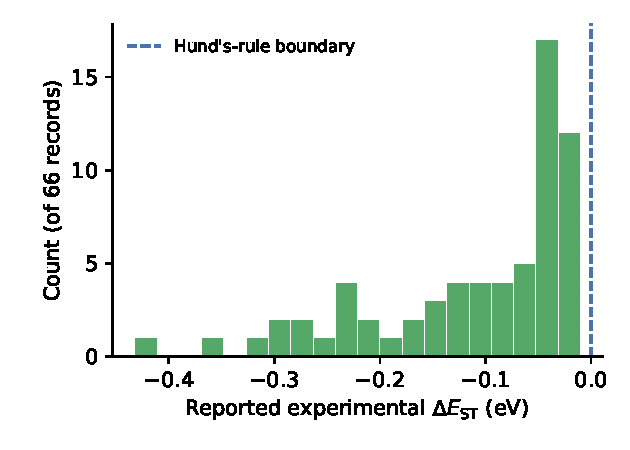
\includegraphics[width=0.72\columnwidth]{figures/ist_delta_est_distribution.pdf}
  \caption{Reported experimental $\Delta E_\text{ST}$ for the \num{66} inverted-gap
    records identified in the literature database. All lie below the Hund's-rule
    boundary (dashed line). Structures were not resolved for these records
    (\texttt{n\_with\_smiles} $=0$), so no model prediction is made for them; they are shown
    to indicate the reported range of the class, not as a test set.}
  \label{fig:istdist}
\end{figure}

\bibliographystyle{elsarticle-num}
\bibliography{references_jmgm}

\end{document}
